\documentclass[1p]{elsarticle_modified}
%\bibliographystyle{elsarticle-num}

%\usepackage[colorlinks]{hyperref}
%\usepackage{abbrmath_seonhwa} %\Abb, \Ascr, \Acal ,\Abf, \Afrak
\usepackage{amsfonts}
\usepackage{amssymb}
\usepackage{amsmath}
\usepackage{amsthm}
\usepackage{scalefnt}
\usepackage{amsbsy}
\usepackage{kotex}
\usepackage{caption}
\usepackage{subfig}
\usepackage{color}
\usepackage{graphicx}
\usepackage{xcolor} %% white, black, red, green, blue, cyan, magenta, yellow
\usepackage{float}
\usepackage{setspace}
\usepackage{hyperref}

\usepackage{tikz}
\usetikzlibrary{arrows}

\usepackage{multirow}
\usepackage{array} % fixed length table
\usepackage{hhline}

%%%%%%%%%%%%%%%%%%%%%
\makeatletter
\renewcommand*\env@matrix[1][\arraystretch]{%
	\edef\arraystretch{#1}%
	\hskip -\arraycolsep
	\let\@ifnextchar\new@ifnextchar
	\array{*\c@MaxMatrixCols c}}
\makeatother %https://tex.stackexchange.com/questions/14071/how-can-i-increase-the-line-spacing-in-a-matrix
%%%%%%%%%%%%%%%

\usepackage[normalem]{ulem}

\newcommand{\msout}[1]{\ifmmode\text{\sout{\ensuremath{#1}}}\else\sout{#1}\fi}
%SOURCE: \msout is \stkout macro in https://tex.stackexchange.com/questions/20609/strikeout-in-math-mode

\newcommand{\cancel}[1]{
	\ifmmode
	{\color{red}\msout{#1}}
	\else
	{\color{red}\sout{#1}}
	\fi
}

\newcommand{\add}[1]{
	{\color{blue}\uwave{#1}}
}

\newcommand{\replace}[2]{
	\ifmmode
	{\color{red}\msout{#1}}{\color{blue}\uwave{#2}}
	\else
	{\color{red}\sout{#1}}{\color{blue}\uwave{#2}}
	\fi
}

\newcommand{\Sol}{\mathcal{S}} %segment
\newcommand{\D}{D} %diagram
\newcommand{\A}{\mathcal{A}} %arc


%%%%%%%%%%%%%%%%%%%%%%%%%%%%%5 test

\def\sl{\operatorname{\textup{SL}}(2,\Cbb)}
\def\psl{\operatorname{\textup{PSL}}(2,\Cbb)}
\def\quan{\mkern 1mu \triangleright \mkern 1mu}

\theoremstyle{definition}
\newtheorem{thm}{Theorem}[section]
\newtheorem{prop}[thm]{Proposition}
\newtheorem{lem}[thm]{Lemma}
\newtheorem{ques}[thm]{Question}
\newtheorem{cor}[thm]{Corollary}
\newtheorem{defn}[thm]{Definition}
\newtheorem{exam}[thm]{Example}
\newtheorem{rmk}[thm]{Remark}
\newtheorem{alg}[thm]{Algorithm}

\newcommand{\I}{\sqrt{-1}}
\begin{document}

%\begin{frontmatter}
%
%\title{Boundary parabolic representations of knots up to 8 crossings}
%
%%% Group authors per affiliation:
%\author{Yunhi Cho} 
%\address{Department of Mathematics, University of Seoul, Seoul, Korea}
%\ead{yhcho@uos.ac.kr}
%
%
%\author{Seonhwa Kim} %\fnref{s_kim}}
%\address{Center for Geometry and Physics, Institute for Basic Science, Pohang, 37673, Korea}
%\ead{ryeona17@ibs.re.kr}
%
%\author{Hyuk Kim}
%\address{Department of Mathematical Sciences, Seoul National University, Seoul 08826, Korea}
%\ead{hyukkim@snu.ac.kr}
%
%\author{Seokbeom Yoon}
%\address{Department of Mathematical Sciences, Seoul National University, Seoul, 08826,  Korea}
%\ead{sbyoon15@snu.ac.kr}
%
%\begin{abstract}
%We find all boundary parabolic representation of knots up to 8 crossings.
%
%\end{abstract}
%\begin{keyword}
%    \MSC[2010] 57M25 
%\end{keyword}
%
%\end{frontmatter}

%\linenumbers
%\tableofcontents
%
\newcommand\colored[1]{\textcolor{white}{\rule[-0.35ex]{0.8em}{1.4ex}}\kern-0.8em\color{red} #1}%
%\newcommand\colored[1]{\textcolor{white}{ #1}\kern-2.17ex	\textcolor{white}{ #1}\kern-1.81ex	\textcolor{white}{ #1}\kern-2.15ex\color{red}#1	}

{\Large $\underline{12a_{0066}~(K12a_{0066})}$}

\setlength{\tabcolsep}{10pt}
\renewcommand{\arraystretch}{1.6}
\vspace{1cm}\begin{tabular}{m{100pt}>{\centering\arraybackslash}m{274pt}}
\multirow{5}{120pt}{
	\centering
	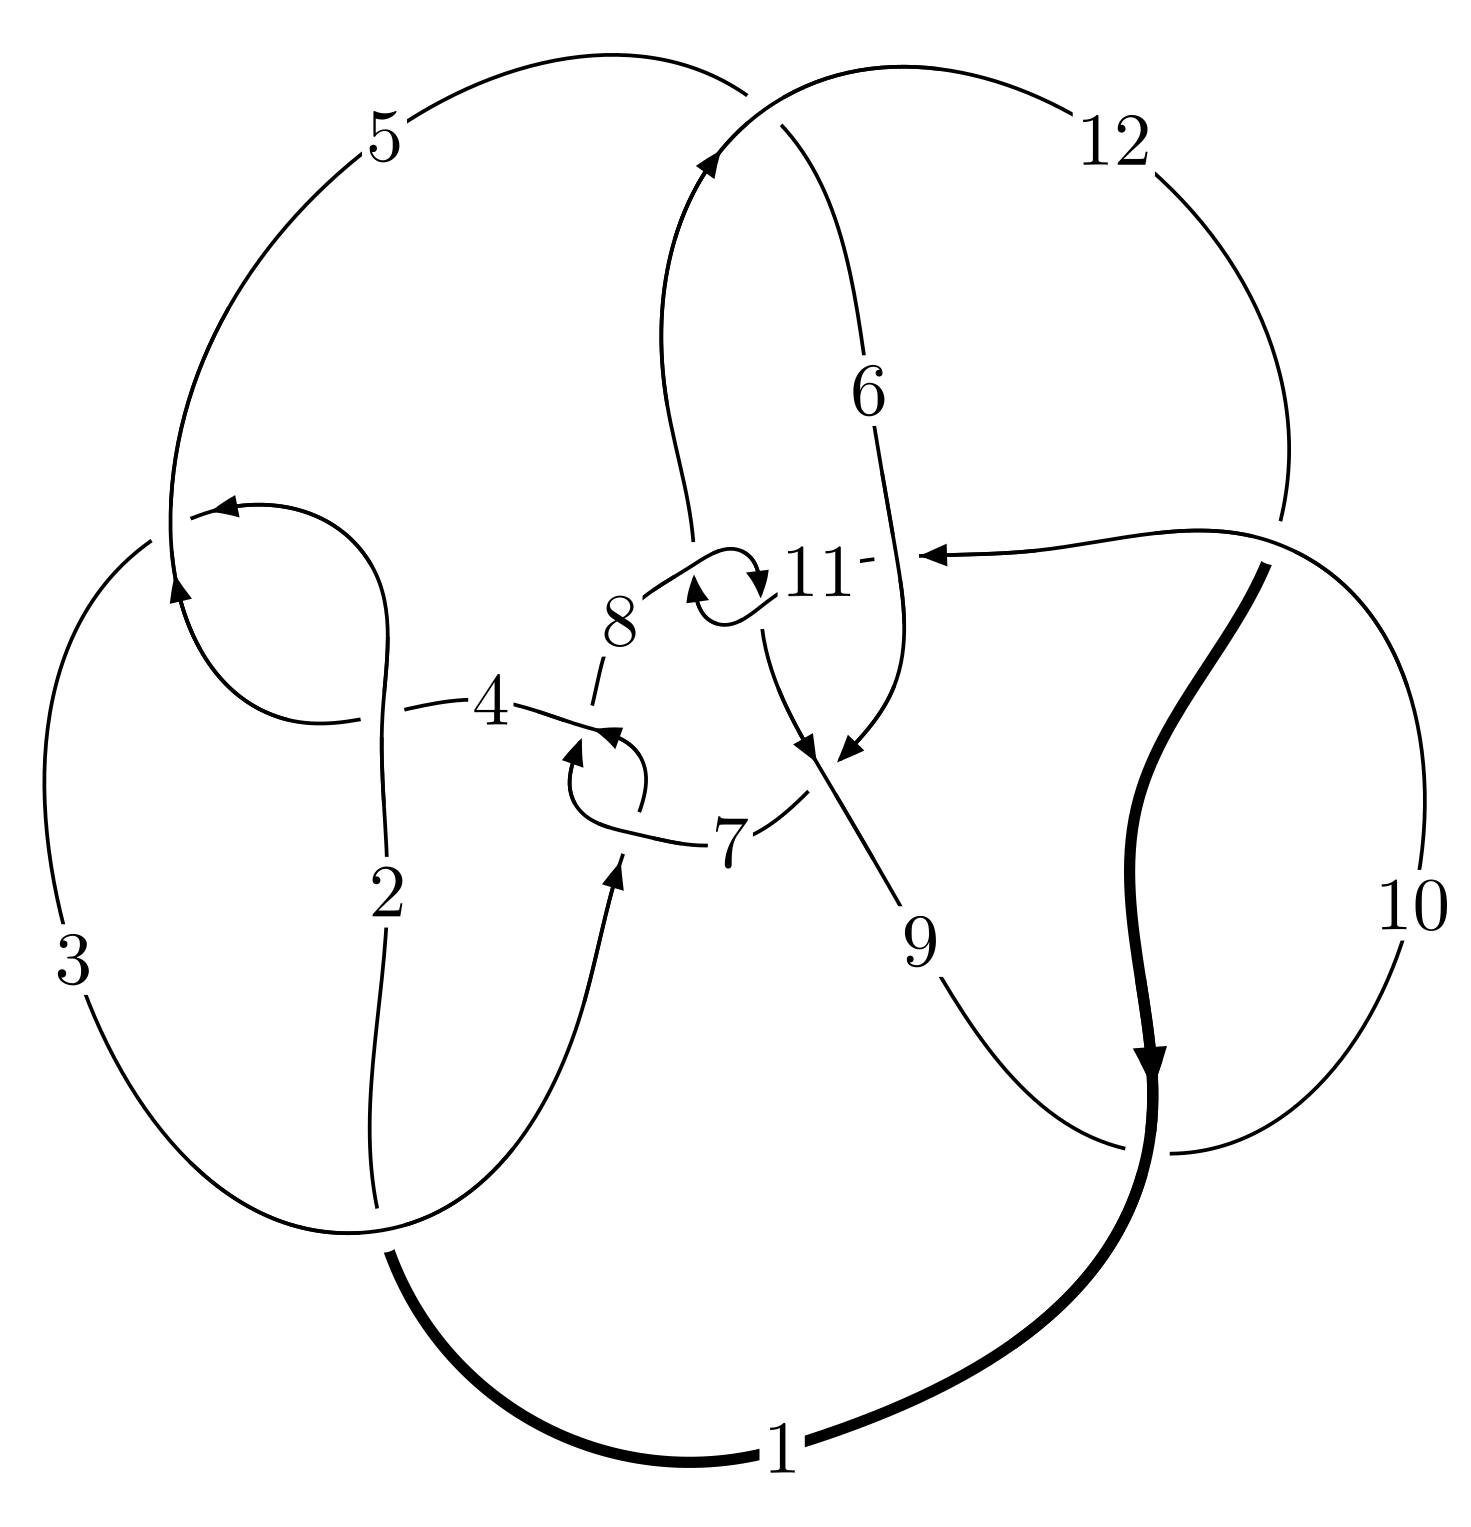
\includegraphics[width=112pt]{../../../GIT/diagram.site/Diagrams/png/867_12a_0066.png}\\
\ \ \ A knot diagram\footnotemark}&
\allowdisplaybreaks
\textbf{Linearized knot diagam} \\
\cline{2-2}
 &
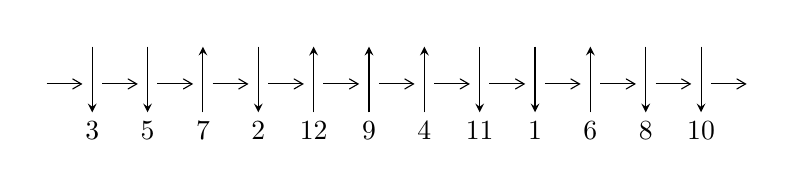
\begin{tikzpicture}[x=20pt, y=17pt]
	% nodes
	\node (C0) at (0, 0) {};
	\node (C1) at (1, 0) {};
	\node (C1U) at (1, +1) {};
	\node (C1D) at (1, -1) {3};

	\node (C2) at (2, 0) {};
	\node (C2U) at (2, +1) {};
	\node (C2D) at (2, -1) {5};

	\node (C3) at (3, 0) {};
	\node (C3U) at (3, +1) {};
	\node (C3D) at (3, -1) {7};

	\node (C4) at (4, 0) {};
	\node (C4U) at (4, +1) {};
	\node (C4D) at (4, -1) {2};

	\node (C5) at (5, 0) {};
	\node (C5U) at (5, +1) {};
	\node (C5D) at (5, -1) {12};

	\node (C6) at (6, 0) {};
	\node (C6U) at (6, +1) {};
	\node (C6D) at (6, -1) {9};

	\node (C7) at (7, 0) {};
	\node (C7U) at (7, +1) {};
	\node (C7D) at (7, -1) {4};

	\node (C8) at (8, 0) {};
	\node (C8U) at (8, +1) {};
	\node (C8D) at (8, -1) {11};

	\node (C9) at (9, 0) {};
	\node (C9U) at (9, +1) {};
	\node (C9D) at (9, -1) {1};

	\node (C10) at (10, 0) {};
	\node (C10U) at (10, +1) {};
	\node (C10D) at (10, -1) {6};

	\node (C11) at (11, 0) {};
	\node (C11U) at (11, +1) {};
	\node (C11D) at (11, -1) {8};

	\node (C12) at (12, 0) {};
	\node (C12U) at (12, +1) {};
	\node (C12D) at (12, -1) {10};
	\node (C13) at (13, 0) {};

	% arrows
	\draw[->,>={angle 60}]
	(C0) edge (C1) (C1) edge (C2) (C2) edge (C3) (C3) edge (C4) (C4) edge (C5) (C5) edge (C6) (C6) edge (C7) (C7) edge (C8) (C8) edge (C9) (C9) edge (C10) (C10) edge (C11) (C11) edge (C12) (C12) edge (C13) ;	\draw[->,>=stealth]
	(C1U) edge (C1D) (C2U) edge (C2D) (C3D) edge (C3U) (C4U) edge (C4D) (C5D) edge (C5U) (C6D) edge (C6U) (C7D) edge (C7U) (C8U) edge (C8D) (C9U) edge (C9D) (C10D) edge (C10U) (C11U) edge (C11D) (C12U) edge (C12D) ;
	\end{tikzpicture} \\
\hhline{~~} \\& 
\textbf{Solving Sequence} \\ \cline{2-2} 
 &
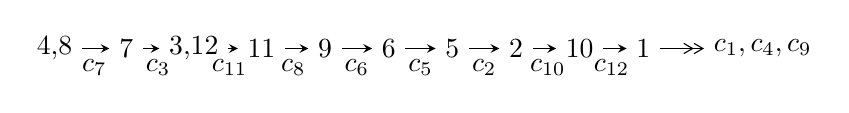
\begin{tikzpicture}[x=23pt, y=7pt]
	% node
	\node (A0) at (-1/8, 0) {4,8};
	\node (A1) at (1, 0) {7};
	\node (A2) at (33/16, 0) {3,12};
	\node (A3) at (25/8, 0) {11};
	\node (A4) at (33/8, 0) {9};
	\node (A5) at (41/8, 0) {6};
	\node (A6) at (49/8, 0) {5};
	\node (A7) at (57/8, 0) {2};
	\node (A8) at (65/8, 0) {10};
	\node (A9) at (73/8, 0) {1};
	\node (C1) at (1/2, -1) {$c_{7}$};
	\node (C2) at (3/2, -1) {$c_{3}$};
	\node (C3) at (21/8, -1) {$c_{11}$};
	\node (C4) at (29/8, -1) {$c_{8}$};
	\node (C5) at (37/8, -1) {$c_{6}$};
	\node (C6) at (45/8, -1) {$c_{5}$};
	\node (C7) at (53/8, -1) {$c_{2}$};
	\node (C8) at (61/8, -1) {$c_{10}$};
	\node (C9) at (69/8, -1) {$c_{12}$};
	\node (A10) at (11, 0) {$c_{1},c_{4},c_{9}$};

	% edge
	\draw[->,>=stealth]	
	(A0) edge (A1) (A1) edge (A2) (A2) edge (A3) (A3) edge (A4) (A4) edge (A5) (A5) edge (A6) (A6) edge (A7) (A7) edge (A8) (A8) edge (A9) ;
	\draw[->>,>={angle 60}]	
	(A9) edge (A10);
\end{tikzpicture} \\ 

\end{tabular} \\

\footnotetext{
The image of knot diagram is generated by the software ``\textbf{Draw programme}" developed by Andrew Bartholomew(\url{http://www.layer8.co.uk/maths/draw/index.htm\#Running-draw}), where we modified some parts for our purpose(\url{https://github.com/CATsTAILs/LinksPainter}).
}\phantom \\ \newline 
\centering \textbf{Ideals for irreducible components\footnotemark of $X_{\text{par}}$} 
 
\begin{align*}
I^u_{1}&=\langle 
6.80476\times10^{108} u^{49}+2.19909\times10^{108} u^{48}+\cdots+1.95260\times10^{111} b-2.72720\times10^{111},\\
\phantom{I^u_{1}}&\phantom{= \langle  }-4.84605\times10^{110} u^{49}-1.94945\times10^{110} u^{48}+\cdots+1.24966\times10^{113} a+4.21327\times10^{112},\\
\phantom{I^u_{1}}&\phantom{= \langle  }u^{50}-12 u^{48}+\cdots+288 u+256\rangle \\
I^u_{2}&=\langle 
-1.95324\times10^{37} a u^{41}+1.89496\times10^{37} u^{41}+\cdots+2.35403\times10^{38} a-3.16022\times10^{38},\\
\phantom{I^u_{2}}&\phantom{= \langle  }1.51510\times10^{33} a u^{41}+3.94443\times10^{33} u^{41}+\cdots-3.53502\times10^{34} a+1.31758\times10^{33},\;u^{42}- u^{41}+\cdots-28 u+8\rangle \\
I^u_{3}&=\langle 
b-1,\;-2 u^5+4 u^3+2 u^2+2 a-4 u+1,\;u^6+u^5- u^4-2 u^3+u+1\rangle \\
\\
I^v_{1}&=\langle 
a,\;4 v^3+7 v^2+3 b+6 v+1,\;4 v^4+7 v^3+2 v^2- v+1\rangle \\
I^v_{2}&=\langle 
a,\;v^2 b+b^2-2 b v+v^2+b- v,\;v^3-2 v^2+v-1\rangle \\
\end{align*}
\raggedright * 5 irreducible components of $\dim_{\mathbb{C}}=0$, with total 150 representations.\\
\footnotetext{All coefficients of polynomials are rational numbers. But the coefficients are sometimes approximated in decimal forms when there is not enough margin.}
\newpage
\renewcommand{\arraystretch}{1}
\centering \section*{I. $I^u_{1}= \langle 6.80\times10^{108} u^{49}+2.20\times10^{108} u^{48}+\cdots+1.95\times10^{111} b-2.73\times10^{111},\;-4.85\times10^{110} u^{49}-1.95\times10^{110} u^{48}+\cdots+1.25\times10^{113} a+4.21\times10^{112},\;u^{50}-12 u^{48}+\cdots+288 u+256 \rangle$}
\flushleft \textbf{(i) Arc colorings}\\
\begin{tabular}{m{7pt} m{180pt} m{7pt} m{180pt} }
\flushright $a_{4}=$&$\begin{pmatrix}0\\u\end{pmatrix}$ \\
\flushright $a_{8}=$&$\begin{pmatrix}1\\0\end{pmatrix}$ \\
\flushright $a_{7}=$&$\begin{pmatrix}1\\u^2\end{pmatrix}$ \\
\flushright $a_{3}=$&$\begin{pmatrix}- u\\- u^3+u\end{pmatrix}$ \\
\flushright $a_{12}=$&$\begin{pmatrix}0.00387789 u^{49}+0.00155998 u^{48}+\cdots+1.14208 u-0.337153\\-0.00348498 u^{49}-0.00112624 u^{48}+\cdots-0.0926115 u+1.39671\end{pmatrix}$ \\
\flushright $a_{11}=$&$\begin{pmatrix}0.000392909 u^{49}+0.000433746 u^{48}+\cdots+1.04946 u+1.05955\\-0.00348498 u^{49}-0.00112624 u^{48}+\cdots-0.0926115 u+1.39671\end{pmatrix}$ \\
\flushright $a_{9}=$&$\begin{pmatrix}0.00111006 u^{49}+0.000131981 u^{48}+\cdots-1.27976 u+0.512699\\0.00140446 u^{49}+0.00290843 u^{48}+\cdots-5.70099 u-1.73217\end{pmatrix}$ \\
\flushright $a_{6}=$&$\begin{pmatrix}0.00201779 u^{49}+0.00143250 u^{48}+\cdots-0.109009 u+0.480487\\-0.00781200 u^{49}-0.00431636 u^{48}+\cdots+5.00237 u+1.88446\end{pmatrix}$ \\
\flushright $a_{5}=$&$\begin{pmatrix}0.00484500 u^{49}-0.000170753 u^{48}+\cdots-3.72519 u-1.11366\\-0.00778716 u^{49}-0.000940792 u^{48}+\cdots+8.29788 u+2.19949\end{pmatrix}$ \\
\flushright $a_{2}=$&$\begin{pmatrix}0.00532065 u^{49}+5.33603\times10^{-6} u^{48}+\cdots-5.76383 u-1.04212\\-0.00949931 u^{49}-0.00114275 u^{48}+\cdots+8.12540 u+2.15441\end{pmatrix}$ \\
\flushright $a_{10}=$&$\begin{pmatrix}0.00121926 u^{49}-0.00119597 u^{48}+\cdots-2.16726 u-0.00363201\\0.00360994 u^{49}+0.00427773 u^{48}+\cdots-1.54167 u+0.244495\end{pmatrix}$ \\
\flushright $a_{1}=$&$\begin{pmatrix}-0.00294216 u^{49}-0.00111155 u^{48}+\cdots+4.57269 u+1.08583\\0.00749971 u^{49}+0.000932472 u^{48}+\cdots-7.22456 u-1.91494\end{pmatrix}$\\&\end{tabular}
\flushleft \textbf{(ii) Obstruction class $= -1$}\\~\\
\flushleft \textbf{(iii) Cusp Shapes $= 0.0110690 u^{49}-0.00700300 u^{48}+\cdots+18.6252 u+7.32722$}\\~\\
\newpage\renewcommand{\arraystretch}{1}
\flushleft \textbf{(iv) u-Polynomials at the component}\newline \\
\begin{tabular}{m{50pt}|m{274pt}}
Crossings & \hspace{64pt}u-Polynomials at each crossing \\
\hline $$\begin{aligned}c_{1}\end{aligned}$$&$\begin{aligned}
&u^{50}+24 u^{49}+\cdots-3807 u+256
\end{aligned}$\\
\hline $$\begin{aligned}c_{2},c_{4}\end{aligned}$$&$\begin{aligned}
&u^{50}-4 u^{49}+\cdots-129 u+16
\end{aligned}$\\
\hline $$\begin{aligned}c_{3},c_{7}\end{aligned}$$&$\begin{aligned}
&u^{50}-12 u^{48}+\cdots+288 u+256
\end{aligned}$\\
\hline $$\begin{aligned}c_{5},c_{6}\end{aligned}$$&$\begin{aligned}
&64(64 u^{50}+160 u^{49}+\cdots+14 u^2+1)
\end{aligned}$\\
\hline $$\begin{aligned}c_{8},c_{9},c_{11}\\c_{12}\end{aligned}$$&$\begin{aligned}
&u^{50}+6 u^{49}+\cdots+2 u+1
\end{aligned}$\\
\hline $$\begin{aligned}c_{10}\end{aligned}$$&$\begin{aligned}
&u^{50}-6 u^{49}+\cdots-94208 u+16384
\end{aligned}$\\
\hline
\end{tabular}\\~\\
\newpage\renewcommand{\arraystretch}{1}
\flushleft \textbf{(v) Riley Polynomials at the component}\newline \\
\begin{tabular}{m{50pt}|m{274pt}}
Crossings & \hspace{64pt}Riley Polynomials at each crossing \\
\hline $$\begin{aligned}c_{1}\end{aligned}$$&$\begin{aligned}
&y^{50}+8 y^{49}+\cdots-4265025 y+65536
\end{aligned}$\\
\hline $$\begin{aligned}c_{2},c_{4}\end{aligned}$$&$\begin{aligned}
&y^{50}-24 y^{49}+\cdots+3807 y+256
\end{aligned}$\\
\hline $$\begin{aligned}c_{3},c_{7}\end{aligned}$$&$\begin{aligned}
&y^{50}-24 y^{49}+\cdots-971776 y+65536
\end{aligned}$\\
\hline $$\begin{aligned}c_{5},c_{6}\end{aligned}$$&$\begin{aligned}
&4096(4096 y^{50}-31744 y^{49}+\cdots+28 y+1)
\end{aligned}$\\
\hline $$\begin{aligned}c_{8},c_{9},c_{11}\\c_{12}\end{aligned}$$&$\begin{aligned}
&y^{50}+22 y^{49}+\cdots+50 y+1
\end{aligned}$\\
\hline $$\begin{aligned}c_{10}\end{aligned}$$&$\begin{aligned}
&y^{50}-14 y^{49}+\cdots-3875536896 y+268435456
\end{aligned}$\\
\hline
\end{tabular}\\~\\
\newpage\flushleft \textbf{(vi) Complex Volumes and Cusp Shapes}
$$\begin{array}{c|c|c}  
\text{Solutions to }I^u_{1}& \I (\text{vol} + \sqrt{-1}CS) & \text{Cusp shape}\\
 \hline 
\begin{aligned}
u &= \phantom{-}0.898117 + 0.279435 I \\
a &= \phantom{-}0.671077 + 0.045381 I \\
b &= -0.247217 - 0.158952 I\end{aligned}
 & \phantom{-}1.50673 + 0.62503 I & \phantom{-}6.47419 - 0.03134 I \\ \hline\begin{aligned}
u &= \phantom{-}0.898117 - 0.279435 I \\
a &= \phantom{-}0.671077 - 0.045381 I \\
b &= -0.247217 + 0.158952 I\end{aligned}
 & \phantom{-}1.50673 - 0.62503 I & \phantom{-}6.47419 + 0.03134 I \\ \hline\begin{aligned}
u &= \phantom{-}0.965194 + 0.442129 I \\
a &= -1.61017 - 0.22648 I \\
b &= \phantom{-}1.071190 - 0.624443 I\end{aligned}
 & -2.71273 + 4.53515 I & -2.87509 - 2.93075 I \\ \hline\begin{aligned}
u &= \phantom{-}0.965194 - 0.442129 I \\
a &= -1.61017 + 0.22648 I \\
b &= \phantom{-}1.071190 + 0.624443 I\end{aligned}
 & -2.71273 - 4.53515 I & -2.87509 + 2.93075 I \\ \hline\begin{aligned}
u &= -0.815600 + 0.692403 I \\
a &= \phantom{-}0.972370 + 0.356228 I \\
b &= -0.469378 - 0.920279 I\end{aligned}
 & -0.49128 - 8.69321 I & -1.67470 + 11.86102 I \\ \hline\begin{aligned}
u &= -0.815600 - 0.692403 I \\
a &= \phantom{-}0.972370 - 0.356228 I \\
b &= -0.469378 + 0.920279 I\end{aligned}
 & -0.49128 + 8.69321 I & -1.67470 - 11.86102 I \\ \hline\begin{aligned}
u &= \phantom{-}0.391611 + 0.792627 I \\
a &= -2.56595 - 0.65373 I \\
b &= \phantom{-}1.172710 - 0.211438 I\end{aligned}
 & -3.48472 - 1.30066 I & \phantom{-}1.53330 + 11.98211 I \\ \hline\begin{aligned}
u &= \phantom{-}0.391611 - 0.792627 I \\
a &= -2.56595 + 0.65373 I \\
b &= \phantom{-}1.172710 + 0.211438 I\end{aligned}
 & -3.48472 + 1.30066 I & \phantom{-}1.53330 - 11.98211 I \\ \hline\begin{aligned}
u &= -1.113190 + 0.328139 I \\
a &= -0.766999 + 0.669164 I \\
b &= \phantom{-}1.346160 - 0.166657 I\end{aligned}
 & \phantom{-}0.75440 - 1.33711 I & \phantom{-}8.60470 + 4.56613 I \\ \hline\begin{aligned}
u &= -1.113190 - 0.328139 I \\
a &= -0.766999 - 0.669164 I \\
b &= \phantom{-}1.346160 + 0.166657 I\end{aligned}
 & \phantom{-}0.75440 + 1.33711 I & \phantom{-}8.60470 - 4.56613 I\\
 \hline 
 \end{array}$$\newpage$$\begin{array}{c|c|c}  
\text{Solutions to }I^u_{1}& \I (\text{vol} + \sqrt{-1}CS) & \text{Cusp shape}\\
 \hline 
\begin{aligned}
u &= -1.003630 + 0.588097 I \\
a &= \phantom{-}0.616489 - 0.235311 I \\
b &= -0.351193 + 0.342652 I\end{aligned}
 & -0.52997 - 5.02287 I & \phantom{-}1.42361 + 2.95767 I \\ \hline\begin{aligned}
u &= -1.003630 - 0.588097 I \\
a &= \phantom{-}0.616489 + 0.235311 I \\
b &= -0.351193 - 0.342652 I\end{aligned}
 & -0.52997 + 5.02287 I & \phantom{-}1.42361 - 2.95767 I \\ \hline\begin{aligned}
u &= \phantom{-}1.112250 + 0.378181 I \\
a &= \phantom{-}1.37497 + 1.15202 I \\
b &= -0.511869 + 1.290650 I\end{aligned}
 & \phantom{-}3.14115 + 10.05270 I & \phantom{-}1.54666 - 6.99924 I \\ \hline\begin{aligned}
u &= \phantom{-}1.112250 - 0.378181 I \\
a &= \phantom{-}1.37497 - 1.15202 I \\
b &= -0.511869 - 1.290650 I\end{aligned}
 & \phantom{-}3.14115 - 10.05270 I & \phantom{-}1.54666 + 6.99924 I \\ \hline\begin{aligned}
u &= -0.195744 + 1.173710 I \\
a &= \phantom{-}0.764863 - 0.753983 I \\
b &= -0.460044 + 1.282800 I\end{aligned}
 & \phantom{-}5.62294 + 7.71288 I & \phantom{-}3.01131 - 4.10494 I \\ \hline\begin{aligned}
u &= -0.195744 - 1.173710 I \\
a &= \phantom{-}0.764863 + 0.753983 I \\
b &= -0.460044 - 1.282800 I\end{aligned}
 & \phantom{-}5.62294 - 7.71288 I & \phantom{-}3.01131 + 4.10494 I \\ \hline\begin{aligned}
u &= -0.778976 + 0.095167 I \\
a &= -1.011110 - 0.147769 I \\
b &= \phantom{-}0.774047 - 0.742819 I\end{aligned}
 & -1.54304 + 0.82047 I & -0.34103 + 1.51386 I \\ \hline\begin{aligned}
u &= -0.778976 - 0.095167 I \\
a &= -1.011110 + 0.147769 I \\
b &= \phantom{-}0.774047 + 0.742819 I\end{aligned}
 & -1.54304 - 0.82047 I & -0.34103 - 1.51386 I \\ \hline\begin{aligned}
u &= \phantom{-}0.546215 + 0.490567 I \\
a &= -0.47633 - 2.47862 I \\
b &= \phantom{-}1.002780 + 0.289724 I\end{aligned}
 & -3.92674 - 0.66017 I & -8.3250 - 13.1911 I \\ \hline\begin{aligned}
u &= \phantom{-}0.546215 - 0.490567 I \\
a &= -0.47633 + 2.47862 I \\
b &= \phantom{-}1.002780 - 0.289724 I\end{aligned}
 & -3.92674 + 0.66017 I & -8.3250 + 13.1911 I\\
 \hline 
 \end{array}$$\newpage$$\begin{array}{c|c|c}  
\text{Solutions to }I^u_{1}& \I (\text{vol} + \sqrt{-1}CS) & \text{Cusp shape}\\
 \hline 
\begin{aligned}
u &= \phantom{-}0.502657 + 1.174230 I \\
a &= \phantom{-}0.840947 + 0.823851 I \\
b &= -0.53623 - 1.31854 I\end{aligned}
 & \phantom{-}4.16035 - 12.95250 I & \phantom{-}0.95450 + 8.17982 I \\ \hline\begin{aligned}
u &= \phantom{-}0.502657 - 1.174230 I \\
a &= \phantom{-}0.840947 - 0.823851 I \\
b &= -0.53623 + 1.31854 I\end{aligned}
 & \phantom{-}4.16035 + 12.95250 I & \phantom{-}0.95450 - 8.17982 I \\ \hline\begin{aligned}
u &= \phantom{-}1.151050 + 0.579567 I \\
a &= -1.12350 - 0.93703 I \\
b &= \phantom{-}1.379840 + 0.292717 I\end{aligned}
 & -1.15010 + 6.50993 I & \phantom{-}2.90407 - 9.24766 I \\ \hline\begin{aligned}
u &= \phantom{-}1.151050 - 0.579567 I \\
a &= -1.12350 + 0.93703 I \\
b &= \phantom{-}1.379840 - 0.292717 I\end{aligned}
 & -1.15010 - 6.50993 I & \phantom{-}2.90407 + 9.24766 I \\ \hline\begin{aligned}
u &= -1.241740 + 0.418945 I \\
a &= \phantom{-}0.523890 - 0.607495 I \\
b &= \phantom{-}0.048258 - 0.824590 I\end{aligned}
 & -1.051330 + 0.854717 I & -9.88678 - 3.08419 I \\ \hline\begin{aligned}
u &= -1.241740 - 0.418945 I \\
a &= \phantom{-}0.523890 + 0.607495 I \\
b &= \phantom{-}0.048258 + 0.824590 I\end{aligned}
 & -1.051330 - 0.854717 I & -9.88678 + 3.08419 I \\ \hline\begin{aligned}
u &= \phantom{-}0.570734 + 0.264073 I \\
a &= \phantom{-}0.981699 + 0.648623 I \\
b &= -0.598386 - 1.137800 I\end{aligned}
 & \phantom{-}1.13411 - 7.11668 I & \phantom{-}4.00252 - 2.15626 I \\ \hline\begin{aligned}
u &= \phantom{-}0.570734 - 0.264073 I \\
a &= \phantom{-}0.981699 - 0.648623 I \\
b &= -0.598386 + 1.137800 I\end{aligned}
 & \phantom{-}1.13411 + 7.11668 I & \phantom{-}4.00252 + 2.15626 I \\ \hline\begin{aligned}
u &= -0.370485 + 0.488941 I \\
a &= \phantom{-}1.40100 + 0.26552 I \\
b &= \phantom{-}0.059670 - 0.170060 I\end{aligned}
 & -1.77807 + 0.66799 I & -4.16532 + 0.83627 I \\ \hline\begin{aligned}
u &= -0.370485 - 0.488941 I \\
a &= \phantom{-}1.40100 - 0.26552 I \\
b &= \phantom{-}0.059670 + 0.170060 I\end{aligned}
 & -1.77807 - 0.66799 I & -4.16532 - 0.83627 I\\
 \hline 
 \end{array}$$\newpage$$\begin{array}{c|c|c}  
\text{Solutions to }I^u_{1}& \I (\text{vol} + \sqrt{-1}CS) & \text{Cusp shape}\\
 \hline 
\begin{aligned}
u &= \phantom{-}0.795488 + 1.154490 I \\
a &= \phantom{-}0.594105 - 0.281157 I \\
b &= -0.222609 + 1.026440 I\end{aligned}
 & \phantom{-}3.64839 + 4.61933 I & \phantom{-}3.31531 - 11.47051 I \\ \hline\begin{aligned}
u &= \phantom{-}0.795488 - 1.154490 I \\
a &= \phantom{-}0.594105 + 0.281157 I \\
b &= -0.222609 - 1.026440 I\end{aligned}
 & \phantom{-}3.64839 - 4.61933 I & \phantom{-}3.31531 + 11.47051 I \\ \hline\begin{aligned}
u &= -0.19057 + 1.41148 I \\
a &= -0.189641 + 0.204297 I \\
b &= \phantom{-}0.183449 - 0.960795 I\end{aligned}
 & \phantom{-}1.12888 + 3.74820 I & \phantom{-0.000000 } 0. - 12.89354 I \\ \hline\begin{aligned}
u &= -0.19057 - 1.41148 I \\
a &= -0.189641 - 0.204297 I \\
b &= \phantom{-}0.183449 + 0.960795 I\end{aligned}
 & \phantom{-}1.12888 - 3.74820 I & \phantom{-0.000000 -}0. + 12.89354 I \\ \hline\begin{aligned}
u &= -1.30509 + 0.60711 I \\
a &= \phantom{-}1.50657 - 0.37542 I \\
b &= -0.55176 - 1.36199 I\end{aligned}
 & \phantom{-}9.1915 - 13.9309 I & \phantom{-0.000000 -}0. + 7.22655 I \\ \hline\begin{aligned}
u &= -1.30509 - 0.60711 I \\
a &= \phantom{-}1.50657 + 0.37542 I \\
b &= -0.55176 + 1.36199 I\end{aligned}
 & \phantom{-}9.1915 + 13.9309 I & \phantom{-0.000000 } 0. - 7.22655 I \\ \hline\begin{aligned}
u &= -0.92121 + 1.12031 I \\
a &= -0.177275 - 0.218827 I \\
b &= -0.126991 + 0.884845 I\end{aligned}
 & -0.38233 + 2.45424 I & \phantom{-0.000000 } 0. - 9.83894 I \\ \hline\begin{aligned}
u &= -0.92121 - 1.12031 I \\
a &= -0.177275 + 0.218827 I \\
b &= -0.126991 - 0.884845 I\end{aligned}
 & -0.38233 - 2.45424 I & \phantom{-0.000000 -}0. + 9.83894 I \\ \hline\begin{aligned}
u &= \phantom{-}1.25070 + 0.75757 I \\
a &= \phantom{-}1.76373 + 0.19301 I \\
b &= -0.59610 + 1.35908 I\end{aligned}
 & \phantom{-}6.5813 + 19.8578 I & \phantom{-0.000000 } 0 \\ \hline\begin{aligned}
u &= \phantom{-}1.25070 - 0.75757 I \\
a &= \phantom{-}1.76373 - 0.19301 I \\
b &= -0.59610 - 1.35908 I\end{aligned}
 & \phantom{-}6.5813 - 19.8578 I & \phantom{-0.000000 } 0\\
 \hline 
 \end{array}$$\newpage$$\begin{array}{c|c|c}  
\text{Solutions to }I^u_{1}& \I (\text{vol} + \sqrt{-1}CS) & \text{Cusp shape}\\
 \hline 
\begin{aligned}
u &= -0.428127 + 0.285395 I \\
a &= -0.800907 + 0.886390 I \\
b &= \phantom{-}0.694592 + 0.408886 I\end{aligned}
 & -1.23082 - 1.07266 I & -4.68345 + 2.46317 I \\ \hline\begin{aligned}
u &= -0.428127 - 0.285395 I \\
a &= -0.800907 - 0.886390 I \\
b &= \phantom{-}0.694592 - 0.408886 I\end{aligned}
 & -1.23082 + 1.07266 I & -4.68345 - 2.46317 I \\ \hline\begin{aligned}
u &= -1.52390 + 0.01972 I \\
a &= \phantom{-}0.334754 - 0.368783 I \\
b &= -0.356016 - 1.353720 I\end{aligned}
 & \phantom{-}12.2277 - 8.7964 I & \phantom{-0.000000 } 0 \\ \hline\begin{aligned}
u &= -1.52390 - 0.01972 I \\
a &= \phantom{-}0.334754 + 0.368783 I \\
b &= -0.356016 + 1.353720 I\end{aligned}
 & \phantom{-}12.2277 + 8.7964 I & \phantom{-0.000000 } 0 \\ \hline\begin{aligned}
u &= -1.35309 + 0.74274 I \\
a &= -1.014570 + 0.310379 I \\
b &= \phantom{-}0.334802 + 1.144640 I\end{aligned}
 & \phantom{-}4.61279 - 11.08970 I & \phantom{-0.000000 } 0 \\ \hline\begin{aligned}
u &= -1.35309 - 0.74274 I \\
a &= -1.014570 - 0.310379 I \\
b &= \phantom{-}0.334802 - 1.144640 I\end{aligned}
 & \phantom{-}4.61279 + 11.08970 I & \phantom{-0.000000 } 0 \\ \hline\begin{aligned}
u &= \phantom{-}1.55085 + 0.24154 I \\
a &= -0.024960 - 0.231338 I \\
b &= -0.262084 - 1.311530 I\end{aligned}
 & \phantom{-}11.83750 - 2.26957 I & \phantom{-0.000000 } 0 \\ \hline\begin{aligned}
u &= \phantom{-}1.55085 - 0.24154 I \\
a &= -0.024960 + 0.231338 I \\
b &= -0.262084 + 1.311530 I\end{aligned}
 & \phantom{-}11.83750 + 2.26957 I & \phantom{-0.000000 } 0 \\ \hline\begin{aligned}
u &= \phantom{-}1.50650 + 0.58645 I \\
a &= -0.663181 - 0.347229 I \\
b &= \phantom{-}0.222382 - 1.119540 I\end{aligned}
 & \phantom{-}7.01611 + 4.67438 I & \phantom{-0.000000 } 0 \\ \hline\begin{aligned}
u &= \phantom{-}1.50650 - 0.58645 I \\
a &= -0.663181 + 0.347229 I \\
b &= \phantom{-}0.222382 + 1.119540 I\end{aligned}
 & \phantom{-}7.01611 - 4.67438 I & \phantom{-0.000000 } 0\\
 \hline 
 \end{array}$$\newpage\newpage\renewcommand{\arraystretch}{1}
\centering \section*{II. $I^u_{2}= \langle -1.95\times10^{37} a u^{41}+1.89\times10^{37} u^{41}+\cdots+2.35\times10^{38} a-3.16\times10^{38},\;1.52\times10^{33} a u^{41}+3.94\times10^{33} u^{41}+\cdots-3.54\times10^{34} a+1.32\times10^{33},\;u^{42}- u^{41}+\cdots-28 u+8 \rangle$}
\flushleft \textbf{(i) Arc colorings}\\
\begin{tabular}{m{7pt} m{180pt} m{7pt} m{180pt} }
\flushright $a_{4}=$&$\begin{pmatrix}0\\u\end{pmatrix}$ \\
\flushright $a_{8}=$&$\begin{pmatrix}1\\0\end{pmatrix}$ \\
\flushright $a_{7}=$&$\begin{pmatrix}1\\u^2\end{pmatrix}$ \\
\flushright $a_{3}=$&$\begin{pmatrix}- u\\- u^3+u\end{pmatrix}$ \\
\flushright $a_{12}=$&$\begin{pmatrix}a\\0.420527 a u^{41}-0.407981 u^{41}+\cdots-5.06818 a+6.80388\end{pmatrix}$ \\
\flushright $a_{11}=$&$\begin{pmatrix}0.420527 a u^{41}-0.407981 u^{41}+\cdots-4.06818 a+6.80388\\0.420527 a u^{41}-0.407981 u^{41}+\cdots-5.06818 a+6.80388\end{pmatrix}$ \\
\flushright $a_{9}=$&$\begin{pmatrix}0.154531 a u^{41}-2.43911 u^{41}+\cdots-3.26279 a+32.6290\\-0.282246 a u^{41}-0.279866 u^{41}+\cdots+1.49713 a+0.975049\end{pmatrix}$ \\
\flushright $a_{6}=$&$\begin{pmatrix}-0.729646 a u^{41}-0.107181 u^{41}+\cdots+11.1484 a-9.07282\\-0.190720 a u^{41}-0.538926 u^{41}+\cdots+1.43722 a+9.71123\end{pmatrix}$ \\
\flushright $a_{5}=$&$\begin{pmatrix}-0.600678 u^{41}+0.244644 u^{40}+\cdots-16.9635 u+8.41409\\-0.578537 u^{41}+0.112322 u^{40}+\cdots-9.27967 u+4.53403\end{pmatrix}$ \\
\flushright $a_{2}=$&$\begin{pmatrix}1.08667 u^{41}-0.309169 u^{40}+\cdots+21.0796 u-10.0999\\0.105021 u^{41}-0.110845 u^{40}+\cdots+8.96049 u-4.53423\end{pmatrix}$ \\
\flushright $a_{10}=$&$\begin{pmatrix}0.407981 a u^{41}-2.35024 u^{41}+\cdots-6.80388 a+31.7051\\-1\end{pmatrix}$ \\
\flushright $a_{1}=$&$\begin{pmatrix}-1.17921 u^{41}+0.356966 u^{40}+\cdots-26.2432 u+12.9481\\0.0287964 u^{41}+0.00828293 u^{40}+\cdots-4.30958 u+2.04396\end{pmatrix}$\\&\end{tabular}
\flushleft \textbf{(ii) Obstruction class $= -1$}\\~\\
\flushleft \textbf{(iii) Cusp Shapes $= 3.13855 u^{41}-0.644766 u^{40}+\cdots+69.1611 u-17.9282$}\\~\\
\newpage\renewcommand{\arraystretch}{1}
\flushleft \textbf{(iv) u-Polynomials at the component}\newline \\
\begin{tabular}{m{50pt}|m{274pt}}
Crossings & \hspace{64pt}u-Polynomials at each crossing \\
\hline $$\begin{aligned}c_{1}\end{aligned}$$&$\begin{aligned}
&(u^{42}+20 u^{41}+\cdots+39 u+1)^{2}
\end{aligned}$\\
\hline $$\begin{aligned}c_{2},c_{4}\end{aligned}$$&$\begin{aligned}
&(u^{42}-4 u^{41}+\cdots+7 u-1)^{2}
\end{aligned}$\\
\hline $$\begin{aligned}c_{3},c_{7}\end{aligned}$$&$\begin{aligned}
&(u^{42}- u^{41}+\cdots-28 u+8)^{2}
\end{aligned}$\\
\hline $$\begin{aligned}c_{5},c_{6}\end{aligned}$$&$\begin{aligned}
&u^{84}+2 u^{83}+\cdots+581438984 u+60886121
\end{aligned}$\\
\hline $$\begin{aligned}c_{8},c_{9},c_{11}\\c_{12}\end{aligned}$$&$\begin{aligned}
&u^{84}-14 u^{83}+\cdots-4 u+1
\end{aligned}$\\
\hline $$\begin{aligned}c_{10}\end{aligned}$$&$\begin{aligned}
&(u^{42}+2 u^{41}+\cdots-2 u-1)^{2}
\end{aligned}$\\
\hline
\end{tabular}\\~\\
\newpage\renewcommand{\arraystretch}{1}
\flushleft \textbf{(v) Riley Polynomials at the component}\newline \\
\begin{tabular}{m{50pt}|m{274pt}}
Crossings & \hspace{64pt}Riley Polynomials at each crossing \\
\hline $$\begin{aligned}c_{1}\end{aligned}$$&$\begin{aligned}
&(y^{42}+8 y^{41}+\cdots-999 y+1)^{2}
\end{aligned}$\\
\hline $$\begin{aligned}c_{2},c_{4}\end{aligned}$$&$\begin{aligned}
&(y^{42}-20 y^{41}+\cdots-39 y+1)^{2}
\end{aligned}$\\
\hline $$\begin{aligned}c_{3},c_{7}\end{aligned}$$&$\begin{aligned}
&(y^{42}-21 y^{41}+\cdots-784 y+64)^{2}
\end{aligned}$\\
\hline $$\begin{aligned}c_{5},c_{6}\end{aligned}$$&$\begin{aligned}
&y^{84}-38 y^{83}+\cdots-58401168007787376 y+3707119730426641
\end{aligned}$\\
\hline $$\begin{aligned}c_{8},c_{9},c_{11}\\c_{12}\end{aligned}$$&$\begin{aligned}
&y^{84}+54 y^{83}+\cdots-60 y^2+1
\end{aligned}$\\
\hline $$\begin{aligned}c_{10}\end{aligned}$$&$\begin{aligned}
&(y^{42}-14 y^{41}+\cdots+2 y+1)^{2}
\end{aligned}$\\
\hline
\end{tabular}\\~\\
\newpage\flushleft \textbf{(vi) Complex Volumes and Cusp Shapes}
$$\begin{array}{c|c|c}  
\text{Solutions to }I^u_{2}& \I (\text{vol} + \sqrt{-1}CS) & \text{Cusp shape}\\
 \hline 
\begin{aligned}
u &= \phantom{-}0.232737 + 0.958770 I \\
a &= \phantom{-}1.51165 - 1.20059 I \\
b &= -0.41354 + 1.37451 I\end{aligned}
 & \phantom{-}4.96975 - 2.03798 I & \phantom{-}4.18964 + 3.67578 I \\ \hline\begin{aligned}
u &= \phantom{-}0.232737 + 0.958770 I \\
a &= \phantom{-}1.47814 + 1.41134 I \\
b &= -0.564224 - 1.240190 I\end{aligned}
 & \phantom{-}4.96975 - 2.03798 I & \phantom{-}4.18964 + 3.67578 I \\ \hline\begin{aligned}
u &= \phantom{-}0.232737 - 0.958770 I \\
a &= \phantom{-}1.51165 + 1.20059 I \\
b &= -0.41354 - 1.37451 I\end{aligned}
 & \phantom{-}4.96975 + 2.03798 I & \phantom{-}4.18964 - 3.67578 I \\ \hline\begin{aligned}
u &= \phantom{-}0.232737 - 0.958770 I \\
a &= \phantom{-}1.47814 - 1.41134 I \\
b &= -0.564224 + 1.240190 I\end{aligned}
 & \phantom{-}4.96975 + 2.03798 I & \phantom{-}4.18964 - 3.67578 I \\ \hline\begin{aligned}
u &= \phantom{-}0.912821 + 0.370122 I \\
a &= \phantom{-}0.081154 + 0.848484 I \\
b &= -0.964211 - 0.072097 I\end{aligned}
 & -0.63969 + 4.75718 I & -1.27952 - 5.86296 I \\ \hline\begin{aligned}
u &= \phantom{-}0.912821 + 0.370122 I \\
a &= -1.76377 - 1.53546 I \\
b &= \phantom{-}0.522152 - 1.265870 I\end{aligned}
 & -0.63969 + 4.75718 I & -1.27952 - 5.86296 I \\ \hline\begin{aligned}
u &= \phantom{-}0.912821 - 0.370122 I \\
a &= \phantom{-}0.081154 - 0.848484 I \\
b &= -0.964211 + 0.072097 I\end{aligned}
 & -0.63969 - 4.75718 I & -1.27952 + 5.86296 I \\ \hline\begin{aligned}
u &= \phantom{-}0.912821 - 0.370122 I \\
a &= -1.76377 + 1.53546 I \\
b &= \phantom{-}0.522152 + 1.265870 I\end{aligned}
 & -0.63969 - 4.75718 I & -1.27952 + 5.86296 I \\ \hline\begin{aligned}
u &= -0.834355 + 0.450716 I \\
a &= \phantom{-}0.496950 - 0.930335 I \\
b &= -0.051378 - 0.222509 I\end{aligned}
 & -1.30280 + 0.70618 I & -3.37702 + 0.55676 I \\ \hline\begin{aligned}
u &= -0.834355 + 0.450716 I \\
a &= \phantom{-}1.80822 - 0.48836 I \\
b &= \phantom{-}0.034418 - 0.871050 I\end{aligned}
 & -1.30280 + 0.70618 I & -3.37702 + 0.55676 I\\
 \hline 
 \end{array}$$\newpage$$\begin{array}{c|c|c}  
\text{Solutions to }I^u_{2}& \I (\text{vol} + \sqrt{-1}CS) & \text{Cusp shape}\\
 \hline 
\begin{aligned}
u &= -0.834355 - 0.450716 I \\
a &= \phantom{-}0.496950 + 0.930335 I \\
b &= -0.051378 + 0.222509 I\end{aligned}
 & -1.30280 - 0.70618 I & -3.37702 - 0.55676 I \\ \hline\begin{aligned}
u &= -0.834355 - 0.450716 I \\
a &= \phantom{-}1.80822 + 0.48836 I \\
b &= \phantom{-}0.034418 + 0.871050 I\end{aligned}
 & -1.30280 - 0.70618 I & -3.37702 - 0.55676 I \\ \hline\begin{aligned}
u &= -0.497589 + 0.958024 I \\
a &= -0.323160 + 0.697370 I \\
b &= \phantom{-}0.183345 + 0.113079 I\end{aligned}
 & -0.62266 + 1.78828 I & -3.96378 - 1.37373 I \\ \hline\begin{aligned}
u &= -0.497589 + 0.958024 I \\
a &= \phantom{-}0.401410 - 0.545035 I \\
b &= -0.107100 + 0.951359 I\end{aligned}
 & -0.62266 + 1.78828 I & -3.96378 - 1.37373 I \\ \hline\begin{aligned}
u &= -0.497589 - 0.958024 I \\
a &= -0.323160 - 0.697370 I \\
b &= \phantom{-}0.183345 - 0.113079 I\end{aligned}
 & -0.62266 - 1.78828 I & -3.96378 + 1.37373 I \\ \hline\begin{aligned}
u &= -0.497589 - 0.958024 I \\
a &= \phantom{-}0.401410 + 0.545035 I \\
b &= -0.107100 - 0.951359 I\end{aligned}
 & -0.62266 - 1.78828 I & -3.96378 + 1.37373 I \\ \hline\begin{aligned}
u &= -0.134308 + 0.909932 I \\
a &= -0.589936 + 1.116220 I \\
b &= \phantom{-}0.411288 - 1.253390 I\end{aligned}
 & \phantom{-}1.66534 + 2.94974 I & \phantom{-}0.00088 - 1.92478 I \\ \hline\begin{aligned}
u &= -0.134308 + 0.909932 I \\
a &= \phantom{-}1.55526 - 0.61214 I \\
b &= -0.848427 + 0.025203 I\end{aligned}
 & \phantom{-}1.66534 + 2.94974 I & \phantom{-}0.00088 - 1.92478 I \\ \hline\begin{aligned}
u &= -0.134308 - 0.909932 I \\
a &= -0.589936 - 1.116220 I \\
b &= \phantom{-}0.411288 + 1.253390 I\end{aligned}
 & \phantom{-}1.66534 - 2.94974 I & \phantom{-}0.00088 + 1.92478 I \\ \hline\begin{aligned}
u &= -0.134308 - 0.909932 I \\
a &= \phantom{-}1.55526 + 0.61214 I \\
b &= -0.848427 - 0.025203 I\end{aligned}
 & \phantom{-}1.66534 - 2.94974 I & \phantom{-}0.00088 + 1.92478 I\\
 \hline 
 \end{array}$$\newpage$$\begin{array}{c|c|c}  
\text{Solutions to }I^u_{2}& \I (\text{vol} + \sqrt{-1}CS) & \text{Cusp shape}\\
 \hline 
\begin{aligned}
u &= \phantom{-}1.086850 + 0.154461 I \\
a &= \phantom{-}0.49387 - 1.92438 I \\
b &= \phantom{-}0.034469 - 1.177150 I\end{aligned}
 & \phantom{-}5.32687 + 0.16365 I & \phantom{-}1.74023 - 0.29295 I \\ \hline\begin{aligned}
u &= \phantom{-}1.086850 + 0.154461 I \\
a &= -1.72226 - 1.23616 I \\
b &= \phantom{-}0.217618 + 0.718151 I\end{aligned}
 & \phantom{-}5.32687 + 0.16365 I & \phantom{-}1.74023 - 0.29295 I \\ \hline\begin{aligned}
u &= \phantom{-}1.086850 - 0.154461 I \\
a &= \phantom{-}0.49387 + 1.92438 I \\
b &= \phantom{-}0.034469 + 1.177150 I\end{aligned}
 & \phantom{-}5.32687 - 0.16365 I & \phantom{-}1.74023 + 0.29295 I \\ \hline\begin{aligned}
u &= \phantom{-}1.086850 - 0.154461 I \\
a &= -1.72226 + 1.23616 I \\
b &= \phantom{-}0.217618 - 0.718151 I\end{aligned}
 & \phantom{-}5.32687 - 0.16365 I & \phantom{-}1.74023 + 0.29295 I \\ \hline\begin{aligned}
u &= -0.798766 + 0.403013 I \\
a &= \phantom{-}1.009400 - 0.071564 I \\
b &= -0.638014 + 0.604613 I\end{aligned}
 & -1.44979 - 4.32552 I & -2.33469 + 7.57694 I \\ \hline\begin{aligned}
u &= -0.798766 + 0.403013 I \\
a &= -0.758354 - 0.408384 I \\
b &= \phantom{-}0.594014 + 0.749718 I\end{aligned}
 & -1.44979 - 4.32552 I & -2.33469 + 7.57694 I \\ \hline\begin{aligned}
u &= -0.798766 - 0.403013 I \\
a &= \phantom{-}1.009400 + 0.071564 I \\
b &= -0.638014 - 0.604613 I\end{aligned}
 & -1.44979 + 4.32552 I & -2.33469 - 7.57694 I \\ \hline\begin{aligned}
u &= -0.798766 - 0.403013 I \\
a &= -0.758354 + 0.408384 I \\
b &= \phantom{-}0.594014 - 0.749718 I\end{aligned}
 & -1.44979 + 4.32552 I & -2.33469 - 7.57694 I \\ \hline\begin{aligned}
u &= \phantom{-}0.465404 + 1.033510 I \\
a &= -0.776621 - 1.132340 I \\
b &= \phantom{-}0.56253 + 1.31912 I\end{aligned}
 & \phantom{-}0.23764 - 7.32917 I & -1.90854 + 6.67478 I \\ \hline\begin{aligned}
u &= \phantom{-}0.465404 + 1.033510 I \\
a &= \phantom{-}1.70092 + 0.38646 I \\
b &= -1.050300 + 0.064111 I\end{aligned}
 & \phantom{-}0.23764 - 7.32917 I & -1.90854 + 6.67478 I\\
 \hline 
 \end{array}$$\newpage$$\begin{array}{c|c|c}  
\text{Solutions to }I^u_{2}& \I (\text{vol} + \sqrt{-1}CS) & \text{Cusp shape}\\
 \hline 
\begin{aligned}
u &= \phantom{-}0.465404 - 1.033510 I \\
a &= -0.776621 + 1.132340 I \\
b &= \phantom{-}0.56253 - 1.31912 I\end{aligned}
 & \phantom{-}0.23764 + 7.32917 I & -1.90854 - 6.67478 I \\ \hline\begin{aligned}
u &= \phantom{-}0.465404 - 1.033510 I \\
a &= \phantom{-}1.70092 - 0.38646 I \\
b &= -1.050300 - 0.064111 I\end{aligned}
 & \phantom{-}0.23764 + 7.32917 I & -1.90854 - 6.67478 I \\ \hline\begin{aligned}
u &= \phantom{-}0.755565 + 0.337157 I \\
a &= -0.856993 - 0.803825 I \\
b &= \phantom{-}0.671995 + 1.050850 I\end{aligned}
 & -1.18242 - 1.63203 I & -1.08702 - 2.62995 I \\ \hline\begin{aligned}
u &= \phantom{-}0.755565 + 0.337157 I \\
a &= \phantom{-}1.399160 + 0.102365 I \\
b &= -0.912786 + 0.392807 I\end{aligned}
 & -1.18242 - 1.63203 I & -1.08702 - 2.62995 I \\ \hline\begin{aligned}
u &= \phantom{-}0.755565 - 0.337157 I \\
a &= -0.856993 + 0.803825 I \\
b &= \phantom{-}0.671995 - 1.050850 I\end{aligned}
 & -1.18242 + 1.63203 I & -1.08702 + 2.62995 I \\ \hline\begin{aligned}
u &= \phantom{-}0.755565 - 0.337157 I \\
a &= \phantom{-}1.399160 - 0.102365 I \\
b &= -0.912786 - 0.392807 I\end{aligned}
 & -1.18242 + 1.63203 I & -1.08702 + 2.62995 I \\ \hline\begin{aligned}
u &= \phantom{-}0.265196 + 0.777853 I \\
a &= -0.132473 + 0.867658 I \\
b &= \phantom{-}0.199134 - 1.031900 I\end{aligned}
 & \phantom{-}1.22766 + 2.20756 I & -0.91183 - 4.39193 I \\ \hline\begin{aligned}
u &= \phantom{-}0.265196 + 0.777853 I \\
a &= \phantom{-}0.798380 - 0.862355 I \\
b &= -0.377178 - 0.039196 I\end{aligned}
 & \phantom{-}1.22766 + 2.20756 I & -0.91183 - 4.39193 I \\ \hline\begin{aligned}
u &= \phantom{-}0.265196 - 0.777853 I \\
a &= -0.132473 - 0.867658 I \\
b &= \phantom{-}0.199134 + 1.031900 I\end{aligned}
 & \phantom{-}1.22766 - 2.20756 I & -0.91183 + 4.39193 I \\ \hline\begin{aligned}
u &= \phantom{-}0.265196 - 0.777853 I \\
a &= \phantom{-}0.798380 + 0.862355 I \\
b &= -0.377178 + 0.039196 I\end{aligned}
 & \phantom{-}1.22766 - 2.20756 I & -0.91183 + 4.39193 I\\
 \hline 
 \end{array}$$\newpage$$\begin{array}{c|c|c}  
\text{Solutions to }I^u_{2}& \I (\text{vol} + \sqrt{-1}CS) & \text{Cusp shape}\\
 \hline 
\begin{aligned}
u &= \phantom{-}0.791058\phantom{ +0.000000I} \\
a &= \phantom{-}0.20284 + 2.66753 I \\
b &= -0.440001 + 1.257300 I\end{aligned}
 & \phantom{-}3.61503\phantom{ +0.000000I} & \phantom{-}7.17890\phantom{ +0.000000I} \\ \hline\begin{aligned}
u &= \phantom{-}0.791058\phantom{ +0.000000I} \\
a &= \phantom{-}0.20284 - 2.66753 I \\
b &= -0.440001 - 1.257300 I\end{aligned}
 & \phantom{-}3.61503\phantom{ +0.000000I} & \phantom{-}7.17890\phantom{ +0.000000I} \\ \hline\begin{aligned}
u &= -1.119440 + 0.484001 I \\
a &= -1.93177 + 0.44893 I \\
b &= \phantom{-}0.291230 - 0.895374 I\end{aligned}
 & \phantom{-}3.92176 - 5.08816 I & -1.48038 + 5.57765 I \\ \hline\begin{aligned}
u &= -1.119440 + 0.484001 I \\
a &= -0.97311 + 1.76409 I \\
b &= \phantom{-}0.122020 + 1.178420 I\end{aligned}
 & \phantom{-}3.92176 - 5.08816 I & -1.48038 + 5.57765 I \\ \hline\begin{aligned}
u &= -1.119440 - 0.484001 I \\
a &= -1.93177 - 0.44893 I \\
b &= \phantom{-}0.291230 + 0.895374 I\end{aligned}
 & \phantom{-}3.92176 + 5.08816 I & -1.48038 - 5.57765 I \\ \hline\begin{aligned}
u &= -1.119440 - 0.484001 I \\
a &= -0.97311 - 1.76409 I \\
b &= \phantom{-}0.122020 - 1.178420 I\end{aligned}
 & \phantom{-}3.92176 + 5.08816 I & -1.48038 - 5.57765 I \\ \hline\begin{aligned}
u &= \phantom{-}1.136730 + 0.486401 I \\
a &= -0.500617 + 0.509781 I \\
b &= \phantom{-}0.353261 - 0.070116 I\end{aligned}
 & \phantom{-}3.85619 + 2.39851 I & \phantom{-}1.004040 - 0.878657 I \\ \hline\begin{aligned}
u &= \phantom{-}1.136730 + 0.486401 I \\
a &= \phantom{-}1.40932 + 0.50529 I \\
b &= -0.158839 + 1.079200 I\end{aligned}
 & \phantom{-}3.85619 + 2.39851 I & \phantom{-}1.004040 - 0.878657 I \\ \hline\begin{aligned}
u &= \phantom{-}1.136730 - 0.486401 I \\
a &= -0.500617 - 0.509781 I \\
b &= \phantom{-}0.353261 + 0.070116 I\end{aligned}
 & \phantom{-}3.85619 - 2.39851 I & \phantom{-}1.004040 + 0.878657 I \\ \hline\begin{aligned}
u &= \phantom{-}1.136730 - 0.486401 I \\
a &= \phantom{-}1.40932 - 0.50529 I \\
b &= -0.158839 - 1.079200 I\end{aligned}
 & \phantom{-}3.85619 - 2.39851 I & \phantom{-}1.004040 + 0.878657 I\\
 \hline 
 \end{array}$$\newpage$$\begin{array}{c|c|c}  
\text{Solutions to }I^u_{2}& \I (\text{vol} + \sqrt{-1}CS) & \text{Cusp shape}\\
 \hline 
\begin{aligned}
u &= \phantom{-}1.207670 + 0.341373 I \\
a &= \phantom{-}0.813751 + 0.915422 I \\
b &= -0.900058 - 0.532369 I\end{aligned}
 & \phantom{-}6.14713 + 1.06689 I & \phantom{-}3.69538 - 0.36183 I \\ \hline\begin{aligned}
u &= \phantom{-}1.207670 + 0.341373 I \\
a &= \phantom{-}0.554985 + 0.079494 I \\
b &= \phantom{-}0.15484 + 1.48362 I\end{aligned}
 & \phantom{-}6.14713 + 1.06689 I & \phantom{-}3.69538 - 0.36183 I \\ \hline\begin{aligned}
u &= \phantom{-}1.207670 - 0.341373 I \\
a &= \phantom{-}0.813751 - 0.915422 I \\
b &= -0.900058 + 0.532369 I\end{aligned}
 & \phantom{-}6.14713 - 1.06689 I & \phantom{-}3.69538 + 0.36183 I \\ \hline\begin{aligned}
u &= \phantom{-}1.207670 - 0.341373 I \\
a &= \phantom{-}0.554985 - 0.079494 I \\
b &= \phantom{-}0.15484 - 1.48362 I\end{aligned}
 & \phantom{-}6.14713 - 1.06689 I & \phantom{-}3.69538 + 0.36183 I \\ \hline\begin{aligned}
u &= -1.263970 + 0.066052 I \\
a &= \phantom{-}0.665062 - 0.472891 I \\
b &= -0.986879 + 0.316168 I\end{aligned}
 & \phantom{-}6.95353 + 4.35155 I & \phantom{-}4.59858 - 5.33139 I \\ \hline\begin{aligned}
u &= -1.263970 + 0.066052 I \\
a &= -0.038901 - 0.425858 I \\
b &= \phantom{-}0.31332 - 1.45728 I\end{aligned}
 & \phantom{-}6.95353 + 4.35155 I & \phantom{-}4.59858 - 5.33139 I \\ \hline\begin{aligned}
u &= -1.263970 - 0.066052 I \\
a &= \phantom{-}0.665062 + 0.472891 I \\
b &= -0.986879 - 0.316168 I\end{aligned}
 & \phantom{-}6.95353 - 4.35155 I & \phantom{-}4.59858 + 5.33139 I \\ \hline\begin{aligned}
u &= -1.263970 - 0.066052 I \\
a &= -0.038901 + 0.425858 I \\
b &= \phantom{-}0.31332 + 1.45728 I\end{aligned}
 & \phantom{-}6.95353 - 4.35155 I & \phantom{-}4.59858 + 5.33139 I \\ \hline\begin{aligned}
u &= -1.253490 + 0.315421 I \\
a &= \phantom{-}1.44870 - 0.39303 I \\
b &= -0.68021 - 1.31927 I\end{aligned}
 & \phantom{-}9.87960 - 1.93798 I & \phantom{-}7.95326 + 1.38361 I \\ \hline\begin{aligned}
u &= -1.253490 + 0.315421 I \\
a &= \phantom{-}0.0176087 + 0.0774925 I \\
b &= -0.46769 + 1.49281 I\end{aligned}
 & \phantom{-}9.87960 - 1.93798 I & \phantom{-}7.95326 + 1.38361 I\\
 \hline 
 \end{array}$$\newpage$$\begin{array}{c|c|c}  
\text{Solutions to }I^u_{2}& \I (\text{vol} + \sqrt{-1}CS) & \text{Cusp shape}\\
 \hline 
\begin{aligned}
u &= -1.253490 - 0.315421 I \\
a &= \phantom{-}1.44870 + 0.39303 I \\
b &= -0.68021 + 1.31927 I\end{aligned}
 & \phantom{-}9.87960 + 1.93798 I & \phantom{-}7.95326 - 1.38361 I \\ \hline\begin{aligned}
u &= -1.253490 - 0.315421 I \\
a &= \phantom{-}0.0176087 - 0.0774925 I \\
b &= -0.46769 - 1.49281 I\end{aligned}
 & \phantom{-}9.87960 + 1.93798 I & \phantom{-}7.95326 - 1.38361 I \\ \hline\begin{aligned}
u &= -0.329380 + 0.607670 I \\
a &= \phantom{-}1.91830 - 6.31824 I \\
b &= \phantom{-}0.045154 - 1.052520 I\end{aligned}
 & \phantom{-}1.56112 + 0.76607 I & -7.12845 - 1.30178 I \\ \hline\begin{aligned}
u &= -0.329380 + 0.607670 I \\
a &= -10.62400 - 2.53492 I \\
b &= \phantom{-}0.061950 + 0.947949 I\end{aligned}
 & \phantom{-}1.56112 + 0.76607 I & -7.12845 - 1.30178 I \\ \hline\begin{aligned}
u &= -0.329380 - 0.607670 I \\
a &= \phantom{-}1.91830 + 6.31824 I \\
b &= \phantom{-}0.045154 + 1.052520 I\end{aligned}
 & \phantom{-}1.56112 - 0.76607 I & -7.12845 + 1.30178 I \\ \hline\begin{aligned}
u &= -0.329380 - 0.607670 I \\
a &= -10.62400 + 2.53492 I \\
b &= \phantom{-}0.061950 - 0.947949 I\end{aligned}
 & \phantom{-}1.56112 - 0.76607 I & -7.12845 + 1.30178 I \\ \hline\begin{aligned}
u &= -1.213380 + 0.511337 I \\
a &= \phantom{-}0.867787 - 0.552784 I \\
b &= -1.143420 + 0.023396 I\end{aligned}
 & \phantom{-}4.97652 - 7.98804 I & \phantom{-}2.75545 + 5.63639 I \\ \hline\begin{aligned}
u &= -1.213380 + 0.511337 I \\
a &= -1.49756 + 0.40473 I \\
b &= \phantom{-}0.58597 + 1.39555 I\end{aligned}
 & \phantom{-}4.97652 - 7.98804 I & \phantom{-}2.75545 + 5.63639 I \\ \hline\begin{aligned}
u &= -1.213380 - 0.511337 I \\
a &= \phantom{-}0.867787 + 0.552784 I \\
b &= -1.143420 - 0.023396 I\end{aligned}
 & \phantom{-}4.97652 + 7.98804 I & \phantom{-}2.75545 - 5.63639 I \\ \hline\begin{aligned}
u &= -1.213380 - 0.511337 I \\
a &= -1.49756 - 0.40473 I \\
b &= \phantom{-}0.58597 - 1.39555 I\end{aligned}
 & \phantom{-}4.97652 + 7.98804 I & \phantom{-}2.75545 - 5.63639 I\\
 \hline 
 \end{array}$$\newpage$$\begin{array}{c|c|c}  
\text{Solutions to }I^u_{2}& \I (\text{vol} + \sqrt{-1}CS) & \text{Cusp shape}\\
 \hline 
\begin{aligned}
u &= -1.165920 + 0.667088 I \\
a &= -0.577892 - 0.133773 I \\
b &= \phantom{-}0.515914 - 0.043918 I\end{aligned}
 & \phantom{-}1.51197 - 7.76497 I & \phantom{-0.000000 -}0. + 4.74518 I \\ \hline\begin{aligned}
u &= -1.165920 + 0.667088 I \\
a &= \phantom{-}1.47345 - 0.28081 I \\
b &= -0.273480 - 1.072760 I\end{aligned}
 & \phantom{-}1.51197 - 7.76497 I & \phantom{-0.000000 -}0. + 4.74518 I \\ \hline\begin{aligned}
u &= -1.165920 - 0.667088 I \\
a &= -0.577892 + 0.133773 I \\
b &= \phantom{-}0.515914 + 0.043918 I\end{aligned}
 & \phantom{-}1.51197 + 7.76497 I & \phantom{-0.000000 } 0. - 4.74518 I \\ \hline\begin{aligned}
u &= -1.165920 - 0.667088 I \\
a &= \phantom{-}1.47345 + 0.28081 I \\
b &= -0.273480 + 1.072760 I\end{aligned}
 & \phantom{-}1.51197 + 7.76497 I & \phantom{-0.000000 } 0. - 4.74518 I \\ \hline\begin{aligned}
u &= \phantom{-}1.239790 + 0.555518 I \\
a &= -0.267910 + 0.337001 I \\
b &= -0.38688 - 1.55484 I\end{aligned}
 & \phantom{-}8.15282 + 7.53350 I & \phantom{-}5.04295 - 6.51119 I \\ \hline\begin{aligned}
u &= \phantom{-}1.239790 + 0.555518 I \\
a &= \phantom{-}1.85937 + 0.13321 I \\
b &= -0.76662 + 1.24734 I\end{aligned}
 & \phantom{-}8.15282 + 7.53350 I & \phantom{-}5.04295 - 6.51119 I \\ \hline\begin{aligned}
u &= \phantom{-}1.239790 - 0.555518 I \\
a &= -0.267910 - 0.337001 I \\
b &= -0.38688 + 1.55484 I\end{aligned}
 & \phantom{-}8.15282 - 7.53350 I & \phantom{-}5.04295 + 6.51119 I \\ \hline\begin{aligned}
u &= \phantom{-}1.239790 - 0.555518 I \\
a &= \phantom{-}1.85937 - 0.13321 I \\
b &= -0.76662 - 1.24734 I\end{aligned}
 & \phantom{-}8.15282 - 7.53350 I & \phantom{-}5.04295 + 6.51119 I \\ \hline\begin{aligned}
u &= \phantom{-}1.205450 + 0.688309 I \\
a &= \phantom{-}1.094510 + 0.734681 I \\
b &= -1.193570 - 0.100733 I\end{aligned}
 & \phantom{-}2.60047 + 13.58860 I & \phantom{-0.000000 } 0. - 9.29837 I \\ \hline\begin{aligned}
u &= \phantom{-}1.205450 + 0.688309 I \\
a &= -1.77964 - 0.13933 I \\
b &= \phantom{-}0.65954 - 1.38657 I\end{aligned}
 & \phantom{-}2.60047 + 13.58860 I & \phantom{-0.000000 } 0. - 9.29837 I\\
 \hline 
 \end{array}$$\newpage$$\begin{array}{c|c|c}  
\text{Solutions to }I^u_{2}& \I (\text{vol} + \sqrt{-1}CS) & \text{Cusp shape}\\
 \hline 
\begin{aligned}
u &= \phantom{-}1.205450 - 0.688309 I \\
a &= \phantom{-}1.094510 - 0.734681 I \\
b &= -1.193570 + 0.100733 I\end{aligned}
 & \phantom{-}2.60047 - 13.58860 I & \phantom{-0.000000 -}0. + 9.29837 I \\ \hline\begin{aligned}
u &= \phantom{-}1.205450 - 0.688309 I \\
a &= -1.77964 + 0.13933 I \\
b &= \phantom{-}0.65954 + 1.38657 I\end{aligned}
 & \phantom{-}2.60047 - 13.58860 I & \phantom{-0.000000 -}0. + 9.29837 I \\ \hline\begin{aligned}
u &= \phantom{-}0.413714\phantom{ +0.000000I} \\
a &= \phantom{-}2.80478 + 2.11582 I \\
b &= -0.209348 - 1.063710 I\end{aligned}
 & \phantom{-}4.17299\phantom{ +0.000000I} & \phantom{-}7.72600\phantom{ +0.000000I} \\ \hline\begin{aligned}
u &= \phantom{-}0.413714\phantom{ +0.000000I} \\
a &= \phantom{-}2.80478 - 2.11582 I \\
b &= -0.209348 + 1.063710 I\end{aligned}
 & \phantom{-}4.17299\phantom{ +0.000000I} & \phantom{-}7.72600\phantom{ +0.000000I}\\
 \hline 
 \end{array}$$\newpage\newpage\renewcommand{\arraystretch}{1}
\centering \section*{III. $I^u_{3}= \langle b-1,\;-2 u^5+4 u^3+2 u^2+2 a-4 u+1,\;u^6+u^5- u^4-2 u^3+u+1 \rangle$}
\flushleft \textbf{(i) Arc colorings}\\
\begin{tabular}{m{7pt} m{180pt} m{7pt} m{180pt} }
\flushright $a_{4}=$&$\begin{pmatrix}0\\u\end{pmatrix}$ \\
\flushright $a_{8}=$&$\begin{pmatrix}1\\0\end{pmatrix}$ \\
\flushright $a_{7}=$&$\begin{pmatrix}1\\u^2\end{pmatrix}$ \\
\flushright $a_{3}=$&$\begin{pmatrix}- u\\- u^3+u\end{pmatrix}$ \\
\flushright $a_{12}=$&$\begin{pmatrix}u^5-2 u^3- u^2+2 u-\frac{1}{2}\\1\end{pmatrix}$ \\
\flushright $a_{11}=$&$\begin{pmatrix}u^5-2 u^3- u^2+2 u+\frac{1}{2}\\1\end{pmatrix}$ \\
\flushright $a_{9}=$&$\begin{pmatrix}u^5-2 u^3- u^2+2 u+\frac{3}{2}\\1\end{pmatrix}$ \\
\flushright $a_{6}=$&$\begin{pmatrix}-\frac{1}{4} u^2+\frac{1}{2}\\\frac{1}{2} u^2\end{pmatrix}$ \\
\flushright $a_{5}=$&$\begin{pmatrix}- u^2+1\\u^2\end{pmatrix}$ \\
\flushright $a_{2}=$&$\begin{pmatrix}- u^4+u^2-1\\u^5+u^4-2 u^3- u^2+u+1\end{pmatrix}$ \\
\flushright $a_{10}=$&$\begin{pmatrix}u^5-2 u^3- u^2+2 u+\frac{1}{2}\\1\end{pmatrix}$ \\
\flushright $a_{1}=$&$\begin{pmatrix}-1\\0\end{pmatrix}$\\&\end{tabular}
\flushleft \textbf{(ii) Obstruction class $= 1$}\\~\\
\flushleft \textbf{(iii) Cusp Shapes $= 4 u^5+\frac{15}{4} u^4-4 u^3-8 u^2+4 u+2$}\\~\\
\newpage\renewcommand{\arraystretch}{1}
\flushleft \textbf{(iv) u-Polynomials at the component}\newline \\
\begin{tabular}{m{50pt}|m{274pt}}
Crossings & \hspace{64pt}u-Polynomials at each crossing \\
\hline $$\begin{aligned}c_{1}\end{aligned}$$&$\begin{aligned}
&u^6-3 u^5+5 u^4-4 u^3+2 u^2- u+1
\end{aligned}$\\
\hline $$\begin{aligned}c_{2},c_{7}\end{aligned}$$&$\begin{aligned}
&u^6+u^5- u^4-2 u^3+u+1
\end{aligned}$\\
\hline $$\begin{aligned}c_{3},c_{4}\end{aligned}$$&$\begin{aligned}
&u^6- u^5- u^4+2 u^3- u+1
\end{aligned}$\\
\hline $$\begin{aligned}c_{5}\end{aligned}$$&$\begin{aligned}
&64(64 u^6-96 u^5+80 u^4-32 u^3+8 u^2-2 u+1)
\end{aligned}$\\
\hline $$\begin{aligned}c_{6}\end{aligned}$$&$\begin{aligned}
&64(64 u^6+96 u^5+80 u^4+32 u^3+8 u^2+2 u+1)
\end{aligned}$\\
\hline $$\begin{aligned}c_{8},c_{9}\end{aligned}$$&$\begin{aligned}
&(u-1)^6
\end{aligned}$\\
\hline $$\begin{aligned}c_{10}\end{aligned}$$&$\begin{aligned}
&u^6
\end{aligned}$\\
\hline $$\begin{aligned}c_{11},c_{12}\end{aligned}$$&$\begin{aligned}
&(u+1)^6
\end{aligned}$\\
\hline
\end{tabular}\\~\\
\newpage\renewcommand{\arraystretch}{1}
\flushleft \textbf{(v) Riley Polynomials at the component}\newline \\
\begin{tabular}{m{50pt}|m{274pt}}
Crossings & \hspace{64pt}Riley Polynomials at each crossing \\
\hline $$\begin{aligned}c_{1}\end{aligned}$$&$\begin{aligned}
&y^6+y^5+5 y^4+6 y^2+3 y+1
\end{aligned}$\\
\hline $$\begin{aligned}c_{2},c_{3},c_{4}\\c_{7}\end{aligned}$$&$\begin{aligned}
&y^6-3 y^5+5 y^4-4 y^3+2 y^2- y+1
\end{aligned}$\\
\hline $$\begin{aligned}c_{5},c_{6}\end{aligned}$$&$\begin{aligned}
&4096(4096 y^6+1024 y^5+1280 y^4+96 y^2+12 y+1)
\end{aligned}$\\
\hline $$\begin{aligned}c_{8},c_{9},c_{11}\\c_{12}\end{aligned}$$&$\begin{aligned}
&(y-1)^6
\end{aligned}$\\
\hline $$\begin{aligned}c_{10}\end{aligned}$$&$\begin{aligned}
&y^6
\end{aligned}$\\
\hline
\end{tabular}\\~\\
\newpage\flushleft \textbf{(vi) Complex Volumes and Cusp Shapes}
$$\begin{array}{c|c|c}  
\text{Solutions to }I^u_{3}& \I (\text{vol} + \sqrt{-1}CS) & \text{Cusp shape}\\
 \hline 
\begin{aligned}
u &= \phantom{-}1.002190 + 0.295542 I \\
a &= -0.730593 - 0.497010 I \\
b &= \phantom{-}1.00000\phantom{ +0.000000I}\end{aligned}
 & \phantom{-}0.245672 + 0.924305 I & -1.78567 + 1.99338 I \\ \hline\begin{aligned}
u &= \phantom{-}1.002190 - 0.295542 I \\
a &= -0.730593 + 0.497010 I \\
b &= \phantom{-}1.00000\phantom{ +0.000000I}\end{aligned}
 & \phantom{-}0.245672 - 0.924305 I & -1.78567 - 1.99338 I \\ \hline\begin{aligned}
u &= -0.428243 + 0.664531 I \\
a &= -2.16103 + 1.45708 I \\
b &= \phantom{-}1.00000\phantom{ +0.000000I}\end{aligned}
 & -3.53554 + 0.92430 I & -0.90787 + 6.83768 I \\ \hline\begin{aligned}
u &= -0.428243 - 0.664531 I \\
a &= -2.16103 - 1.45708 I \\
b &= \phantom{-}1.00000\phantom{ +0.000000I}\end{aligned}
 & -3.53554 - 0.92430 I & -0.90787 - 6.83768 I \\ \hline\begin{aligned}
u &= -1.073950 + 0.558752 I \\
a &= -1.108380 + 0.558752 I \\
b &= \phantom{-}1.00000\phantom{ +0.000000I}\end{aligned}
 & -1.64493 - 5.69302 I & -3.18146 + 4.26477 I \\ \hline\begin{aligned}
u &= -1.073950 - 0.558752 I \\
a &= -1.108380 - 0.558752 I \\
b &= \phantom{-}1.00000\phantom{ +0.000000I}\end{aligned}
 & -1.64493 + 5.69302 I & -3.18146 - 4.26477 I\\
 \hline 
 \end{array}$$\newpage\newpage\renewcommand{\arraystretch}{1}
\centering \section*{IV. $I^v_{1}= \langle a,\;4 v^3+7 v^2+3 b+6 v+1,\;4 v^4+7 v^3+2 v^2- v+1 \rangle$}
\flushleft \textbf{(i) Arc colorings}\\
\begin{tabular}{m{7pt} m{180pt} m{7pt} m{180pt} }
\flushright $a_{4}=$&$\begin{pmatrix}v\\0\end{pmatrix}$ \\
\flushright $a_{8}=$&$\begin{pmatrix}1\\0\end{pmatrix}$ \\
\flushright $a_{7}=$&$\begin{pmatrix}1\\0\end{pmatrix}$ \\
\flushright $a_{3}=$&$\begin{pmatrix}v\\0\end{pmatrix}$ \\
\flushright $a_{12}=$&$\begin{pmatrix}0\\-\frac{4}{3} v^3-\frac{7}{3} v^2-2 v-\frac{1}{3}\end{pmatrix}$ \\
\flushright $a_{11}=$&$\begin{pmatrix}-\frac{4}{3} v^3-\frac{7}{3} v^2-2 v-\frac{1}{3}\\-\frac{4}{3} v^3-\frac{7}{3} v^2-2 v-\frac{1}{3}\end{pmatrix}$ \\
\flushright $a_{9}=$&$\begin{pmatrix}\frac{4}{3} v^3+\frac{11}{3} v^2+\frac{5}{3} v\\\frac{4}{3} v^3+\frac{11}{3} v^2+\frac{5}{3} v-1\end{pmatrix}$ \\
\flushright $a_{6}=$&$\begin{pmatrix}-\frac{4}{3} v^3-\frac{7}{3} v^2-2 v-\frac{1}{3}\\-\frac{8}{3} v^3-6 v^2-\frac{11}{3} v-\frac{1}{3}\end{pmatrix}$ \\
\flushright $a_{5}=$&$\begin{pmatrix}-\frac{4}{3} v^3-\frac{7}{3} v^2-2 v-\frac{1}{3}\\-4 v^3-7 v^2-2 v+1\end{pmatrix}$ \\
\flushright $a_{2}=$&$\begin{pmatrix}\frac{4}{3} v^3+\frac{7}{3} v^2+3 v+\frac{1}{3}\\4 v^3+7 v^2+2 v-1\end{pmatrix}$ \\
\flushright $a_{10}=$&$\begin{pmatrix}1\\\frac{8}{3} v^2+\frac{10}{3} v+\frac{4}{3}\end{pmatrix}$ \\
\flushright $a_{1}=$&$\begin{pmatrix}\frac{4}{3} v^3+\frac{7}{3} v^2+2 v+\frac{1}{3}\\4 v^3+7 v^2+2 v-1\end{pmatrix}$\\&\end{tabular}
\flushleft \textbf{(ii) Obstruction class $= 1$}\\~\\
\flushleft \textbf{(iii) Cusp Shapes $= 4 v^3+\frac{62}{3} v^2+\frac{67}{3} v-\frac{11}{3}$}\\~\\
\newpage\renewcommand{\arraystretch}{1}
\flushleft \textbf{(iv) u-Polynomials at the component}\newline \\
\begin{tabular}{m{50pt}|m{274pt}}
Crossings & \hspace{64pt}u-Polynomials at each crossing \\
\hline $$\begin{aligned}c_{1},c_{2}\end{aligned}$$&$\begin{aligned}
&(u-1)^4
\end{aligned}$\\
\hline $$\begin{aligned}c_{3},c_{7}\end{aligned}$$&$\begin{aligned}
&u^4
\end{aligned}$\\
\hline $$\begin{aligned}c_{4}\end{aligned}$$&$\begin{aligned}
&(u+1)^4
\end{aligned}$\\
\hline $$\begin{aligned}c_{5},c_{6}\end{aligned}$$&$\begin{aligned}
&u^4+2 u^3+3 u^2+u+1
\end{aligned}$\\
\hline $$\begin{aligned}c_{8},c_{9}\end{aligned}$$&$\begin{aligned}
&u^4+u^2- u+1
\end{aligned}$\\
\hline $$\begin{aligned}c_{10}\end{aligned}$$&$\begin{aligned}
&u^4+3 u^3+4 u^2+3 u+2
\end{aligned}$\\
\hline $$\begin{aligned}c_{11},c_{12}\end{aligned}$$&$\begin{aligned}
&u^4+u^2+u+1
\end{aligned}$\\
\hline
\end{tabular}\\~\\
\newpage\renewcommand{\arraystretch}{1}
\flushleft \textbf{(v) Riley Polynomials at the component}\newline \\
\begin{tabular}{m{50pt}|m{274pt}}
Crossings & \hspace{64pt}Riley Polynomials at each crossing \\
\hline $$\begin{aligned}c_{1},c_{2},c_{4}\end{aligned}$$&$\begin{aligned}
&(y-1)^4
\end{aligned}$\\
\hline $$\begin{aligned}c_{3},c_{7}\end{aligned}$$&$\begin{aligned}
&y^4
\end{aligned}$\\
\hline $$\begin{aligned}c_{5},c_{6}\end{aligned}$$&$\begin{aligned}
&y^4+2 y^3+7 y^2+5 y+1
\end{aligned}$\\
\hline $$\begin{aligned}c_{8},c_{9},c_{11}\\c_{12}\end{aligned}$$&$\begin{aligned}
&y^4+2 y^3+3 y^2+y+1
\end{aligned}$\\
\hline $$\begin{aligned}c_{10}\end{aligned}$$&$\begin{aligned}
&y^4- y^3+2 y^2+7 y+4
\end{aligned}$\\
\hline
\end{tabular}\\~\\
\newpage\flushleft \textbf{(vi) Complex Volumes and Cusp Shapes}
$$\begin{array}{c|c|c}  
\text{Solutions to }I^v_{1}& \I (\text{vol} + \sqrt{-1}CS) & \text{Cusp shape}\\
 \hline 
\begin{aligned}
v &= -1.112690 + 0.371716 I \\
a &= \phantom{-0.000000 } 0 \\
b &= \phantom{-}0.547424 - 0.585652 I\end{aligned}
 & -2.62503 + 1.39709 I & -9.45081 - 3.47689 I \\ \hline\begin{aligned}
v &= -1.112690 - 0.371716 I \\
a &= \phantom{-0.000000 } 0 \\
b &= \phantom{-}0.547424 + 0.585652 I\end{aligned}
 & -2.62503 - 1.39709 I & -9.45081 + 3.47689 I \\ \hline\begin{aligned}
v &= \phantom{-}0.237691 + 0.353773 I \\
a &= \phantom{-0.000000 } 0 \\
b &= -0.547424 - 1.120870 I\end{aligned}
 & \phantom{-}0.98010 - 7.64338 I & -0.08044 + 11.43934 I \\ \hline\begin{aligned}
v &= \phantom{-}0.237691 - 0.353773 I \\
a &= \phantom{-0.000000 } 0 \\
b &= -0.547424 + 1.120870 I\end{aligned}
 & \phantom{-}0.98010 + 7.64338 I & -0.08044 - 11.43934 I\\
 \hline 
 \end{array}$$\newpage\newpage\renewcommand{\arraystretch}{1}
\centering \section*{V. $I^v_{2}= \langle a,\;v^2 b+b^2-2 b v+v^2+b- v,\;v^3-2 v^2+v-1 \rangle$}
\flushleft \textbf{(i) Arc colorings}\\
\begin{tabular}{m{7pt} m{180pt} m{7pt} m{180pt} }
\flushright $a_{4}=$&$\begin{pmatrix}v\\0\end{pmatrix}$ \\
\flushright $a_{8}=$&$\begin{pmatrix}1\\0\end{pmatrix}$ \\
\flushright $a_{7}=$&$\begin{pmatrix}1\\0\end{pmatrix}$ \\
\flushright $a_{3}=$&$\begin{pmatrix}v\\0\end{pmatrix}$ \\
\flushright $a_{12}=$&$\begin{pmatrix}0\\b\end{pmatrix}$ \\
\flushright $a_{11}=$&$\begin{pmatrix}b\\b\end{pmatrix}$ \\
\flushright $a_{9}=$&$\begin{pmatrix}- v^2 b+2 b v- v^2- b+v+1\\- v^2 b+2 b v- v^2- b+v\end{pmatrix}$ \\
\flushright $a_{6}=$&$\begin{pmatrix}b v- b+1\\v^2 b- b v+v^2- v\end{pmatrix}$ \\
\flushright $a_{5}=$&$\begin{pmatrix}b v- b+1\\v^2-2 v+1\end{pmatrix}$ \\
\flushright $a_{2}=$&$\begin{pmatrix}- b v+b+v-1\\- v^2+2 v-1\end{pmatrix}$ \\
\flushright $a_{10}=$&$\begin{pmatrix}- v^2 b+2 b v- v+1\\-1\end{pmatrix}$ \\
\flushright $a_{1}=$&$\begin{pmatrix}- b v+b-1\\- v^2+2 v-1\end{pmatrix}$\\&\end{tabular}
\flushleft \textbf{(ii) Obstruction class $= 1$}\\~\\
\flushleft \textbf{(iii) Cusp Shapes $= -2 v^2+5 v-5$}\\~\\
\newpage\renewcommand{\arraystretch}{1}
\flushleft \textbf{(iv) u-Polynomials at the component}\newline \\
\begin{tabular}{m{50pt}|m{274pt}}
Crossings & \hspace{64pt}u-Polynomials at each crossing \\
\hline $$\begin{aligned}c_{1},c_{2}\end{aligned}$$&$\begin{aligned}
&(u-1)^6
\end{aligned}$\\
\hline $$\begin{aligned}c_{3},c_{7}\end{aligned}$$&$\begin{aligned}
&u^6
\end{aligned}$\\
\hline $$\begin{aligned}c_{4}\end{aligned}$$&$\begin{aligned}
&(u+1)^6
\end{aligned}$\\
\hline $$\begin{aligned}c_{5},c_{6}\end{aligned}$$&$\begin{aligned}
&u^6+3 u^5+4 u^4+2 u^3+1
\end{aligned}$\\
\hline $$\begin{aligned}c_{8},c_{9}\end{aligned}$$&$\begin{aligned}
&u^6+u^5+2 u^4+2 u^3+2 u^2+2 u+1
\end{aligned}$\\
\hline $$\begin{aligned}c_{10}\end{aligned}$$&$\begin{aligned}
&(u^3- u^2+1)^2
\end{aligned}$\\
\hline $$\begin{aligned}c_{11},c_{12}\end{aligned}$$&$\begin{aligned}
&u^6- u^5+2 u^4-2 u^3+2 u^2-2 u+1
\end{aligned}$\\
\hline
\end{tabular}\\~\\
\newpage\renewcommand{\arraystretch}{1}
\flushleft \textbf{(v) Riley Polynomials at the component}\newline \\
\begin{tabular}{m{50pt}|m{274pt}}
Crossings & \hspace{64pt}Riley Polynomials at each crossing \\
\hline $$\begin{aligned}c_{1},c_{2},c_{4}\end{aligned}$$&$\begin{aligned}
&(y-1)^6
\end{aligned}$\\
\hline $$\begin{aligned}c_{3},c_{7}\end{aligned}$$&$\begin{aligned}
&y^6
\end{aligned}$\\
\hline $$\begin{aligned}c_{5},c_{6}\end{aligned}$$&$\begin{aligned}
&y^6- y^5+4 y^4-2 y^3+8 y^2+1
\end{aligned}$\\
\hline $$\begin{aligned}c_{8},c_{9},c_{11}\\c_{12}\end{aligned}$$&$\begin{aligned}
&y^6+3 y^5+4 y^4+2 y^3+1
\end{aligned}$\\
\hline $$\begin{aligned}c_{10}\end{aligned}$$&$\begin{aligned}
&(y^3- y^2+2 y-1)^2
\end{aligned}$\\
\hline
\end{tabular}\\~\\
\newpage\flushleft \textbf{(vi) Complex Volumes and Cusp Shapes}
$$\begin{array}{c|c|c}  
\text{Solutions to }I^v_{2}& \I (\text{vol} + \sqrt{-1}CS) & \text{Cusp shape}\\
 \hline 
\begin{aligned}
v &= \phantom{-}0.122561 + 0.744862 I \\
a &= \phantom{-0.000000 } 0 \\
b &= \phantom{-}0.498832 + 1.001300 I\end{aligned}
 & -1.37919 - 2.82812 I & -3.30760 + 3.35914 I \\ \hline\begin{aligned}
v &= \phantom{-}0.122561 + 0.744862 I \\
a &= \phantom{-0.000000 } 0 \\
b &= -0.713912 + 0.305839 I\end{aligned}
 & -1.37919 - 2.82812 I & -3.30760 + 3.35914 I \\ \hline\begin{aligned}
v &= \phantom{-}0.122561 - 0.744862 I \\
a &= \phantom{-0.000000 } 0 \\
b &= \phantom{-}0.498832 - 1.001300 I\end{aligned}
 & -1.37919 + 2.82812 I & -3.30760 - 3.35914 I \\ \hline\begin{aligned}
v &= \phantom{-}0.122561 - 0.744862 I \\
a &= \phantom{-0.000000 } 0 \\
b &= -0.713912 - 0.305839 I\end{aligned}
 & -1.37919 + 2.82812 I & -3.30760 - 3.35914 I \\ \hline\begin{aligned}
v &= \phantom{-}1.75488\phantom{ +0.000000I} \\
a &= \phantom{-0.000000 } 0 \\
b &= -0.284920 + 1.115140 I\end{aligned}
 & \phantom{-}2.75839\phantom{ +0.000000I} & -2.38480\phantom{ +0.000000I} \\ \hline\begin{aligned}
v &= \phantom{-}1.75488\phantom{ +0.000000I} \\
a &= \phantom{-0.000000 } 0 \\
b &= -0.284920 - 1.115140 I\end{aligned}
 & \phantom{-}2.75839\phantom{ +0.000000I} & -2.38480\phantom{ +0.000000I}\\
 \hline 
 \end{array}$$\newpage
\newpage\renewcommand{\arraystretch}{1}
\centering \section*{ VI. u-Polynomials}
\begin{tabular}{m{50pt}|m{274pt}}
Crossings & \hspace{64pt}u-Polynomials at each crossing \\
\hline $$\begin{aligned}c_{1}\end{aligned}$$&$\begin{aligned}
&(u-1)^{10}(u^6-3 u^5+5 u^4-4 u^3+2 u^2- u+1)\\
&\cdot((u^{42}+20 u^{41}+\cdots+39 u+1)^{2})(u^{50}+24 u^{49}+\cdots-3807 u+256)
\end{aligned}$\\
\hline $$\begin{aligned}c_{2}\end{aligned}$$&$\begin{aligned}
&((u-1)^{10})(u^6+u^5+\cdots+u+1)(u^{42}-4 u^{41}+\cdots+7 u-1)^{2}\\
&\cdot(u^{50}-4 u^{49}+\cdots-129 u+16)
\end{aligned}$\\
\hline $$\begin{aligned}c_{3}\end{aligned}$$&$\begin{aligned}
&u^{10}(u^6- u^5+\cdots- u+1)(u^{42}- u^{41}+\cdots-28 u+8)^{2}\\
&\cdot(u^{50}-12 u^{48}+\cdots+288 u+256)
\end{aligned}$\\
\hline $$\begin{aligned}c_{4}\end{aligned}$$&$\begin{aligned}
&((u+1)^{10})(u^6- u^5+\cdots- u+1)(u^{42}-4 u^{41}+\cdots+7 u-1)^{2}\\
&\cdot(u^{50}-4 u^{49}+\cdots-129 u+16)
\end{aligned}$\\
\hline $$\begin{aligned}c_{5}\end{aligned}$$&$\begin{aligned}
&4096(u^4+2 u^3+3 u^2+u+1)(u^6+3 u^5+4 u^4+2 u^3+1)\\
&\cdot(64 u^6-96 u^5+80 u^4-32 u^3+8 u^2-2 u+1)\\
&\cdot(64 u^{50}+160 u^{49}+\cdots+14 u^2+1)\\
&\cdot(u^{84}+2 u^{83}+\cdots+581438984 u+60886121)
\end{aligned}$\\
\hline $$\begin{aligned}c_{6}\end{aligned}$$&$\begin{aligned}
&4096(u^4+2 u^3+3 u^2+u+1)(u^6+3 u^5+4 u^4+2 u^3+1)\\
&\cdot(64 u^6+96 u^5+80 u^4+32 u^3+8 u^2+2 u+1)\\
&\cdot(64 u^{50}+160 u^{49}+\cdots+14 u^2+1)\\
&\cdot(u^{84}+2 u^{83}+\cdots+581438984 u+60886121)
\end{aligned}$\\
\hline $$\begin{aligned}c_{7}\end{aligned}$$&$\begin{aligned}
&u^{10}(u^6+u^5+\cdots+u+1)(u^{42}- u^{41}+\cdots-28 u+8)^{2}\\
&\cdot(u^{50}-12 u^{48}+\cdots+288 u+256)
\end{aligned}$\\
\hline $$\begin{aligned}c_{8},c_{9}\end{aligned}$$&$\begin{aligned}
&(u-1)^6(u^4+u^2- u+1)(u^6+u^5+2 u^4+2 u^3+2 u^2+2 u+1)\\
&\cdot(u^{50}+6 u^{49}+\cdots+2 u+1)(u^{84}-14 u^{83}+\cdots-4 u+1)
\end{aligned}$\\
\hline $$\begin{aligned}c_{10}\end{aligned}$$&$\begin{aligned}
&u^6(u^3- u^2+1)^2(u^{4}+3 u^{3}+\cdots+3 u+2)(u^{42}+2 u^{41}+\cdots-2 u-1)^{2}\\
&\cdot(u^{50}-6 u^{49}+\cdots-94208 u+16384)
\end{aligned}$\\
\hline $$\begin{aligned}c_{11},c_{12}\end{aligned}$$&$\begin{aligned}
&(u+1)^6(u^4+u^2+u+1)(u^6- u^5+2 u^4-2 u^3+2 u^2-2 u+1)\\
&\cdot(u^{50}+6 u^{49}+\cdots+2 u+1)(u^{84}-14 u^{83}+\cdots-4 u+1)
\end{aligned}$\\
\hline
\end{tabular}\newpage\renewcommand{\arraystretch}{1}
\centering \section*{ VII. Riley Polynomials}
\begin{tabular}{m{50pt}|m{274pt}}
Crossings & \hspace{64pt}Riley Polynomials at each crossing \\
\hline $$\begin{aligned}c_{1}\end{aligned}$$&$\begin{aligned}
&((y-1)^{10})(y^6+y^5+\cdots+3 y+1)(y^{42}+8 y^{41}+\cdots-999 y+1)^{2}\\
&\cdot(y^{50}+8 y^{49}+\cdots-4265025 y+65536)
\end{aligned}$\\
\hline $$\begin{aligned}c_{2},c_{4}\end{aligned}$$&$\begin{aligned}
&(y-1)^{10}(y^6-3 y^5+5 y^4-4 y^3+2 y^2- y+1)\\
&\cdot((y^{42}-20 y^{41}+\cdots-39 y+1)^{2})(y^{50}-24 y^{49}+\cdots+3807 y+256)
\end{aligned}$\\
\hline $$\begin{aligned}c_{3},c_{7}\end{aligned}$$&$\begin{aligned}
&y^{10}(y^6-3 y^5+5 y^4-4 y^3+2 y^2- y+1)\\
&\cdot(y^{42}-21 y^{41}+\cdots-784 y+64)^{2}\\
&\cdot(y^{50}-24 y^{49}+\cdots-971776 y+65536)
\end{aligned}$\\
\hline $$\begin{aligned}c_{5},c_{6}\end{aligned}$$&$\begin{aligned}
&16777216(y^4+2 y^3+7 y^2+5 y+1)(y^6- y^5+4 y^4-2 y^3+8 y^2+1)\\
&\cdot(4096 y^6+1024 y^5+1280 y^4+96 y^2+12 y+1)\\
&\cdot(4096 y^{50}-31744 y^{49}+\cdots+28 y+1)\\
&\cdot(y^{84}-38 y^{83}+\cdots-58401168007787376 y+3707119730426641)
\end{aligned}$\\
\hline $$\begin{aligned}c_{8},c_{9},c_{11}\\c_{12}\end{aligned}$$&$\begin{aligned}
&(y-1)^6(y^4+2 y^3+3 y^2+y+1)(y^6+3 y^5+4 y^4+2 y^3+1)\\
&\cdot(y^{50}+22 y^{49}+\cdots+50 y+1)(y^{84}+54 y^{83}+\cdots-60 y^2+1)
\end{aligned}$\\
\hline $$\begin{aligned}c_{10}\end{aligned}$$&$\begin{aligned}
&y^6(y^3- y^2+2 y-1)^2(y^4- y^3+2 y^2+7 y+4)\\
&\cdot(y^{42}-14 y^{41}+\cdots+2 y+1)^{2}\\
&\cdot(y^{50}-14 y^{49}+\cdots-3875536896 y+268435456)
\end{aligned}$\\
\hline
\end{tabular}
\vskip 2pc
\end{document}